\documentclass[1p]{elsarticle_modified}
%\bibliographystyle{elsarticle-num}

%\usepackage[colorlinks]{hyperref}
%\usepackage{abbrmath_seonhwa} %\Abb, \Ascr, \Acal ,\Abf, \Afrak
\usepackage{amsfonts}
\usepackage{amssymb}
\usepackage{amsmath}
\usepackage{amsthm}
\usepackage{scalefnt}
\usepackage{amsbsy}
\usepackage{kotex}
\usepackage{caption}
\usepackage{subfig}
\usepackage{color}
\usepackage{graphicx}
\usepackage{xcolor} %% white, black, red, green, blue, cyan, magenta, yellow
\usepackage{float}
\usepackage{setspace}
\usepackage{hyperref}

\usepackage{tikz}
\usetikzlibrary{arrows}

\usepackage{multirow}
\usepackage{array} % fixed length table
\usepackage{hhline}

%%%%%%%%%%%%%%%%%%%%%
\makeatletter
\renewcommand*\env@matrix[1][\arraystretch]{%
	\edef\arraystretch{#1}%
	\hskip -\arraycolsep
	\let\@ifnextchar\new@ifnextchar
	\array{*\c@MaxMatrixCols c}}
\makeatother %https://tex.stackexchange.com/questions/14071/how-can-i-increase-the-line-spacing-in-a-matrix
%%%%%%%%%%%%%%%

\usepackage[normalem]{ulem}

\newcommand{\msout}[1]{\ifmmode\text{\sout{\ensuremath{#1}}}\else\sout{#1}\fi}
%SOURCE: \msout is \stkout macro in https://tex.stackexchange.com/questions/20609/strikeout-in-math-mode

\newcommand{\cancel}[1]{
	\ifmmode
	{\color{red}\msout{#1}}
	\else
	{\color{red}\sout{#1}}
	\fi
}

\newcommand{\add}[1]{
	{\color{blue}\uwave{#1}}
}

\newcommand{\replace}[2]{
	\ifmmode
	{\color{red}\msout{#1}}{\color{blue}\uwave{#2}}
	\else
	{\color{red}\sout{#1}}{\color{blue}\uwave{#2}}
	\fi
}

\newcommand{\Sol}{\mathcal{S}} %segment
\newcommand{\D}{D} %diagram
\newcommand{\A}{\mathcal{A}} %arc


%%%%%%%%%%%%%%%%%%%%%%%%%%%%%5 test

\def\sl{\operatorname{\textup{SL}}(2,\Cbb)}
\def\psl{\operatorname{\textup{PSL}}(2,\Cbb)}
\def\quan{\mkern 1mu \triangleright \mkern 1mu}

\theoremstyle{definition}
\newtheorem{thm}{Theorem}[section]
\newtheorem{prop}[thm]{Proposition}
\newtheorem{lem}[thm]{Lemma}
\newtheorem{ques}[thm]{Question}
\newtheorem{cor}[thm]{Corollary}
\newtheorem{defn}[thm]{Definition}
\newtheorem{exam}[thm]{Example}
\newtheorem{rmk}[thm]{Remark}
\newtheorem{alg}[thm]{Algorithm}

\newcommand{\I}{\sqrt{-1}}
\begin{document}

%\begin{frontmatter}
%
%\title{Boundary parabolic representations of knots up to 8 crossings}
%
%%% Group authors per affiliation:
%\author{Yunhi Cho} 
%\address{Department of Mathematics, University of Seoul, Seoul, Korea}
%\ead{yhcho@uos.ac.kr}
%
%
%\author{Seonhwa Kim} %\fnref{s_kim}}
%\address{Center for Geometry and Physics, Institute for Basic Science, Pohang, 37673, Korea}
%\ead{ryeona17@ibs.re.kr}
%
%\author{Hyuk Kim}
%\address{Department of Mathematical Sciences, Seoul National University, Seoul 08826, Korea}
%\ead{hyukkim@snu.ac.kr}
%
%\author{Seokbeom Yoon}
%\address{Department of Mathematical Sciences, Seoul National University, Seoul, 08826,  Korea}
%\ead{sbyoon15@snu.ac.kr}
%
%\begin{abstract}
%We find all boundary parabolic representation of knots up to 8 crossings.
%
%\end{abstract}
%\begin{keyword}
%    \MSC[2010] 57M25 
%\end{keyword}
%
%\end{frontmatter}

%\linenumbers
%\tableofcontents
%
\newcommand\colored[1]{\textcolor{white}{\rule[-0.35ex]{0.8em}{1.4ex}}\kern-0.8em\color{red} #1}%
%\newcommand\colored[1]{\textcolor{white}{ #1}\kern-2.17ex	\textcolor{white}{ #1}\kern-1.81ex	\textcolor{white}{ #1}\kern-2.15ex\color{red}#1	}

{\Large $\underline{12a_{0629}~(K12a_{0629})}$}

\setlength{\tabcolsep}{10pt}
\renewcommand{\arraystretch}{1.6}
\vspace{1cm}\begin{tabular}{m{100pt}>{\centering\arraybackslash}m{274pt}}
\multirow{5}{120pt}{
	\centering
	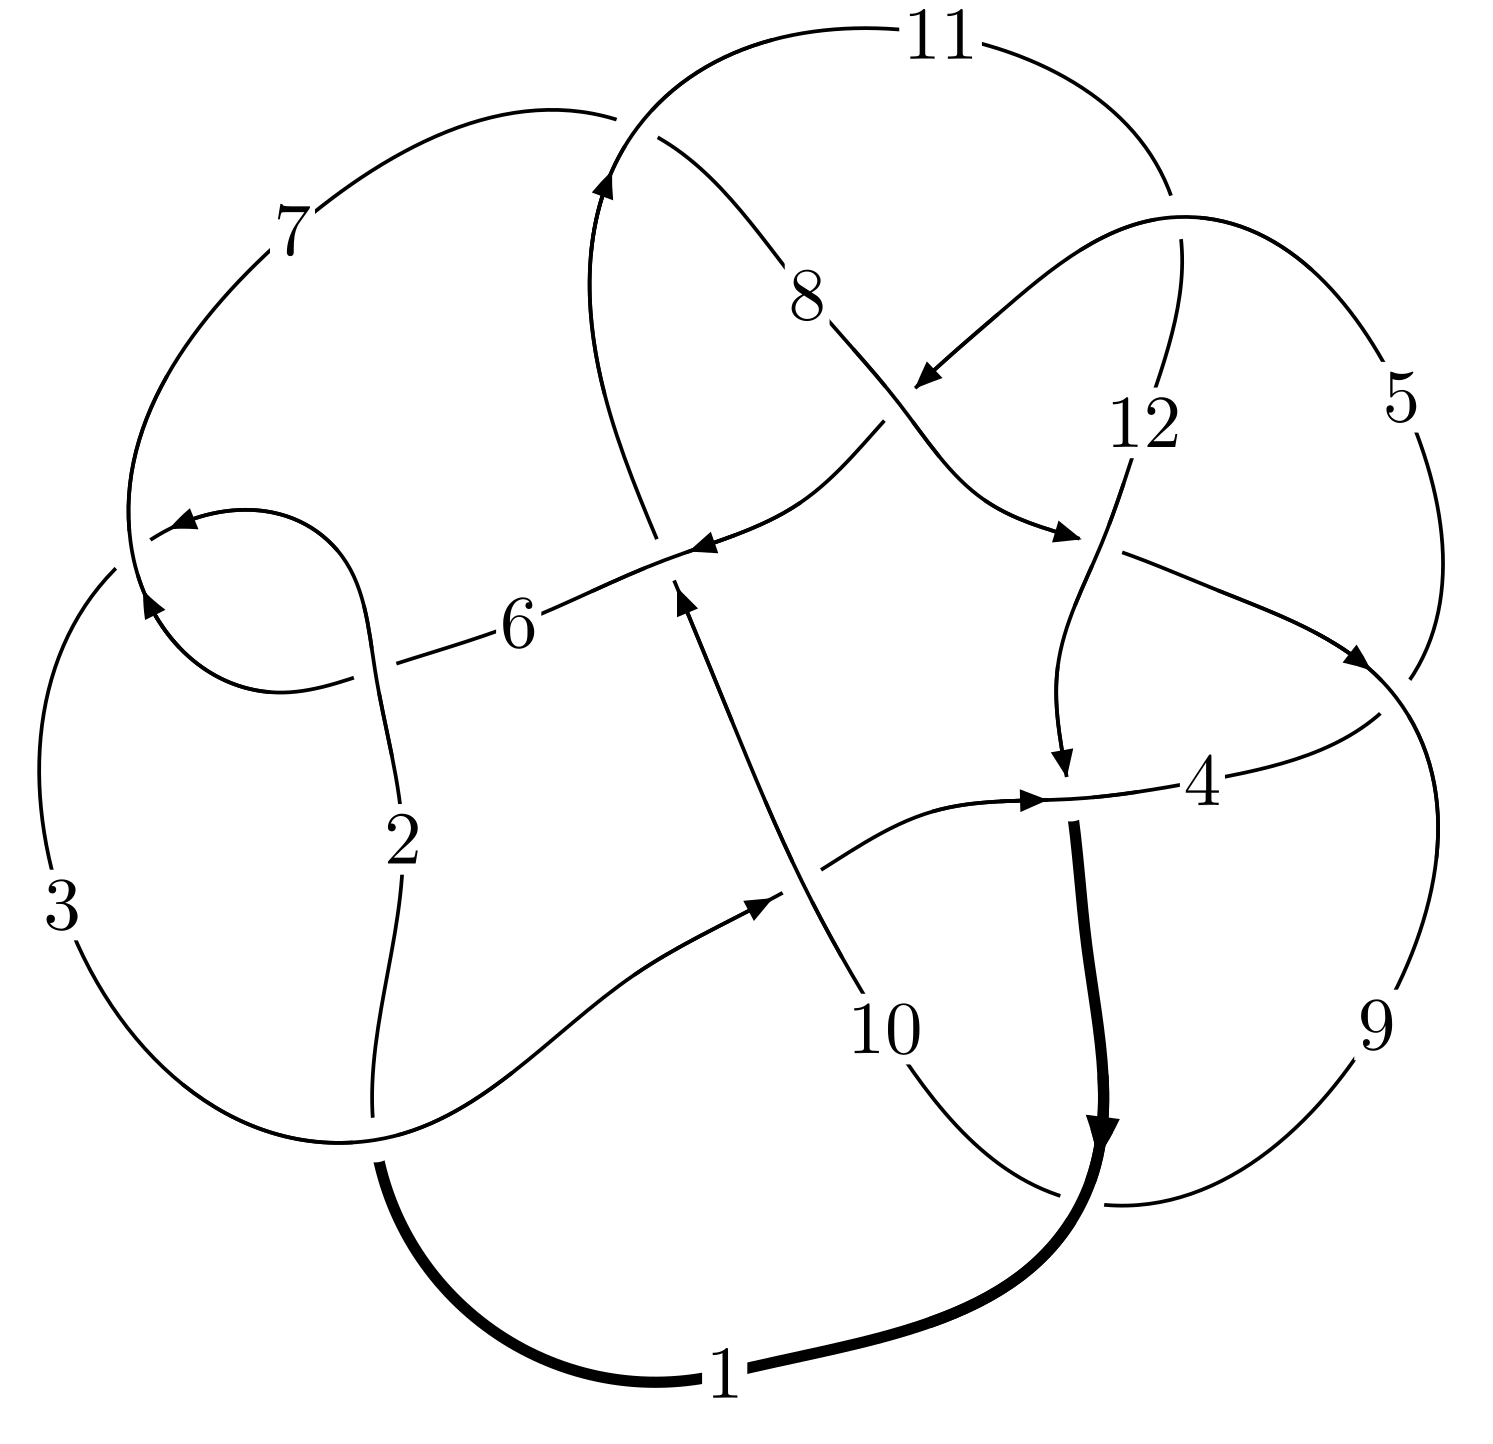
\includegraphics[width=112pt]{../../../GIT/diagram.site/Diagrams/png/1430_12a_0629.png}\\
\ \ \ A knot diagram\footnotemark}&
\allowdisplaybreaks
\textbf{Linearized knot diagam} \\
\cline{2-2}
 &
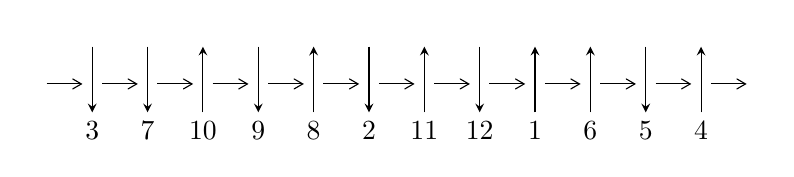
\begin{tikzpicture}[x=20pt, y=17pt]
	% nodes
	\node (C0) at (0, 0) {};
	\node (C1) at (1, 0) {};
	\node (C1U) at (1, +1) {};
	\node (C1D) at (1, -1) {3};

	\node (C2) at (2, 0) {};
	\node (C2U) at (2, +1) {};
	\node (C2D) at (2, -1) {7};

	\node (C3) at (3, 0) {};
	\node (C3U) at (3, +1) {};
	\node (C3D) at (3, -1) {10};

	\node (C4) at (4, 0) {};
	\node (C4U) at (4, +1) {};
	\node (C4D) at (4, -1) {9};

	\node (C5) at (5, 0) {};
	\node (C5U) at (5, +1) {};
	\node (C5D) at (5, -1) {8};

	\node (C6) at (6, 0) {};
	\node (C6U) at (6, +1) {};
	\node (C6D) at (6, -1) {2};

	\node (C7) at (7, 0) {};
	\node (C7U) at (7, +1) {};
	\node (C7D) at (7, -1) {11};

	\node (C8) at (8, 0) {};
	\node (C8U) at (8, +1) {};
	\node (C8D) at (8, -1) {12};

	\node (C9) at (9, 0) {};
	\node (C9U) at (9, +1) {};
	\node (C9D) at (9, -1) {1};

	\node (C10) at (10, 0) {};
	\node (C10U) at (10, +1) {};
	\node (C10D) at (10, -1) {6};

	\node (C11) at (11, 0) {};
	\node (C11U) at (11, +1) {};
	\node (C11D) at (11, -1) {5};

	\node (C12) at (12, 0) {};
	\node (C12U) at (12, +1) {};
	\node (C12D) at (12, -1) {4};
	\node (C13) at (13, 0) {};

	% arrows
	\draw[->,>={angle 60}]
	(C0) edge (C1) (C1) edge (C2) (C2) edge (C3) (C3) edge (C4) (C4) edge (C5) (C5) edge (C6) (C6) edge (C7) (C7) edge (C8) (C8) edge (C9) (C9) edge (C10) (C10) edge (C11) (C11) edge (C12) (C12) edge (C13) ;	\draw[->,>=stealth]
	(C1U) edge (C1D) (C2U) edge (C2D) (C3D) edge (C3U) (C4U) edge (C4D) (C5D) edge (C5U) (C6U) edge (C6D) (C7D) edge (C7U) (C8U) edge (C8D) (C9D) edge (C9U) (C10D) edge (C10U) (C11U) edge (C11D) (C12D) edge (C12U) ;
	\end{tikzpicture} \\
\hhline{~~} \\& 
\textbf{Solving Sequence} \\ \cline{2-2} 
 &
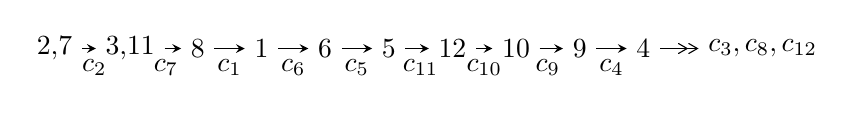
\begin{tikzpicture}[x=23pt, y=7pt]
	% node
	\node (A0) at (-1/8, 0) {2,7};
	\node (A1) at (17/16, 0) {3,11};
	\node (A2) at (17/8, 0) {8};
	\node (A3) at (25/8, 0) {1};
	\node (A4) at (33/8, 0) {6};
	\node (A5) at (41/8, 0) {5};
	\node (A6) at (49/8, 0) {12};
	\node (A7) at (57/8, 0) {10};
	\node (A8) at (65/8, 0) {9};
	\node (A9) at (73/8, 0) {4};
	\node (C1) at (1/2, -1) {$c_{2}$};
	\node (C2) at (13/8, -1) {$c_{7}$};
	\node (C3) at (21/8, -1) {$c_{1}$};
	\node (C4) at (29/8, -1) {$c_{6}$};
	\node (C5) at (37/8, -1) {$c_{5}$};
	\node (C6) at (45/8, -1) {$c_{11}$};
	\node (C7) at (53/8, -1) {$c_{10}$};
	\node (C8) at (61/8, -1) {$c_{9}$};
	\node (C9) at (69/8, -1) {$c_{4}$};
	\node (A10) at (11, 0) {$c_{3},c_{8},c_{12}$};

	% edge
	\draw[->,>=stealth]	
	(A0) edge (A1) (A1) edge (A2) (A2) edge (A3) (A3) edge (A4) (A4) edge (A5) (A5) edge (A6) (A6) edge (A7) (A7) edge (A8) (A8) edge (A9) ;
	\draw[->>,>={angle 60}]	
	(A9) edge (A10);
\end{tikzpicture} \\ 

\end{tabular} \\

\footnotetext{
The image of knot diagram is generated by the software ``\textbf{Draw programme}" developed by Andrew Bartholomew(\url{http://www.layer8.co.uk/maths/draw/index.htm\#Running-draw}), where we modified some parts for our purpose(\url{https://github.com/CATsTAILs/LinksPainter}).
}\phantom \\ \newline 
\centering \textbf{Ideals for irreducible components\footnotemark of $X_{\text{par}}$} 
 
\begin{align*}
I^u_{1}&=\langle 
8556215038 u^{35}+88954311703 u^{34}+\cdots+896216536 b+256623421136,\\
\phantom{I^u_{1}}&\phantom{= \langle  }7106105223 u^{35}+72031097023 u^{34}+\cdots+1792433072 a+143687532288,\\
\phantom{I^u_{1}}&\phantom{= \langle  }u^{36}+11 u^{35}+\cdots+272 u+32\rangle \\
I^u_{2}&=\langle 
-11687 u^{23}+18829 u^{22}+\cdots+10412 b+20692,\;-10340 u^{23}+11229 u^{22}+\cdots+5206 a+1655,\\
\phantom{I^u_{2}}&\phantom{= \langle  }u^{24}-2 u^{23}+\cdots-3 u+1\rangle \\
I^u_{3}&=\langle 
-8 u^{67} a-1512 u^{67}+\cdots+8 a-1868,\;511 u^{67} a+3 u^{67}+\cdots+443 a+3488,\;u^{68}-6 u^{67}+\cdots-11 u-1\rangle \\
\\
\end{align*}
\raggedright * 3 irreducible components of $\dim_{\mathbb{C}}=0$, with total 196 representations.\\
\footnotetext{All coefficients of polynomials are rational numbers. But the coefficients are sometimes approximated in decimal forms when there is not enough margin.}
\newpage
\renewcommand{\arraystretch}{1}
\centering \section*{I. $I^u_{1}= \langle 8.56\times10^{9} u^{35}+8.90\times10^{10} u^{34}+\cdots+8.96\times10^{8} b+2.57\times10^{11},\;7.11\times10^{9} u^{35}+7.20\times10^{10} u^{34}+\cdots+1.79\times10^{9} a+1.44\times10^{11},\;u^{36}+11 u^{35}+\cdots+272 u+32 \rangle$}
\flushleft \textbf{(i) Arc colorings}\\
\begin{tabular}{m{7pt} m{180pt} m{7pt} m{180pt} }
\flushright $a_{2}=$&$\begin{pmatrix}1\\0\end{pmatrix}$ \\
\flushright $a_{7}=$&$\begin{pmatrix}0\\u\end{pmatrix}$ \\
\flushright $a_{3}=$&$\begin{pmatrix}1\\u^2\end{pmatrix}$ \\
\flushright $a_{11}=$&$\begin{pmatrix}-3.96450 u^{35}-40.1862 u^{34}+\cdots-651.842 u-80.1634\\-9.54704 u^{35}-99.2554 u^{34}+\cdots-2249.93 u-286.341\end{pmatrix}$ \\
\flushright $a_{8}=$&$\begin{pmatrix}-6.08616 u^{35}-59.5811 u^{34}+\cdots-971.052 u-121.494\\-9.21243 u^{35}-90.5844 u^{34}+\cdots-1619.60 u-203.975\end{pmatrix}$ \\
\flushright $a_{1}=$&$\begin{pmatrix}- u^2+1\\- u^4\end{pmatrix}$ \\
\flushright $a_{6}=$&$\begin{pmatrix}u\\u\end{pmatrix}$ \\
\flushright $a_{5}=$&$\begin{pmatrix}4.05928 u^{35}+48.5520 u^{34}+\cdots+1754.80 u+230.994\\3.45731 u^{35}+47.7820 u^{34}+\cdots+2476.13 u+333.311\end{pmatrix}$ \\
\flushright $a_{12}=$&$\begin{pmatrix}3.69166 u^{35}+29.8903 u^{34}+\cdots-157.090 u-25.3283\\12.5638 u^{35}+116.784 u^{34}+\cdots+1115.12 u+127.351\end{pmatrix}$ \\
\flushright $a_{10}=$&$\begin{pmatrix}-6.60941 u^{35}-60.5115 u^{34}+\cdots-194.344 u-5.32351\\-12.1919 u^{35}-119.581 u^{34}+\cdots-1792.43 u-211.501\end{pmatrix}$ \\
\flushright $a_{9}=$&$\begin{pmatrix}7.05419 u^{35}+69.3065 u^{34}+\cdots+1216.08 u+157.152\\17.2900 u^{35}+178.333 u^{34}+\cdots+3753.55 u+479.519\end{pmatrix}$ \\
\flushright $a_{4}=$&$\begin{pmatrix}16.4473 u^{35}+145.651 u^{34}+\cdots-514.224 u-124.290\\35.2687 u^{35}+346.194 u^{34}+\cdots+4598.95 u+526.313\end{pmatrix}$\\&\end{tabular}
\flushleft \textbf{(ii) Obstruction class $= -1$}\\~\\
\flushleft \textbf{(iii) Cusp Shapes $= -\frac{37524040947}{224054134} u^{35}-\frac{350685729393}{224054134} u^{34}+\cdots-\frac{964109017840}{112027067} u-\frac{73536479818}{112027067}$}\\~\\
\newpage\renewcommand{\arraystretch}{1}
\flushleft \textbf{(iv) u-Polynomials at the component}\newline \\
\begin{tabular}{m{50pt}|m{274pt}}
Crossings & \hspace{64pt}u-Polynomials at each crossing \\
\hline $$\begin{aligned}c_{1}\end{aligned}$$&$\begin{aligned}
&u^{36}+11 u^{35}+\cdots-4352 u+1024
\end{aligned}$\\
\hline $$\begin{aligned}c_{2},c_{6}\end{aligned}$$&$\begin{aligned}
&u^{36}-11 u^{35}+\cdots-272 u+32
\end{aligned}$\\
\hline $$\begin{aligned}c_{3},c_{10}\end{aligned}$$&$\begin{aligned}
&u^{36}+6 u^{35}+\cdots+2 u+2
\end{aligned}$\\
\hline $$\begin{aligned}c_{4},c_{11}\end{aligned}$$&$\begin{aligned}
&u^{36}+6 u^{35}+\cdots- u+1
\end{aligned}$\\
\hline $$\begin{aligned}c_{5},c_{12}\end{aligned}$$&$\begin{aligned}
&u^{36}+2 u^{35}+\cdots+8 u+1
\end{aligned}$\\
\hline $$\begin{aligned}c_{7},c_{9}\end{aligned}$$&$\begin{aligned}
&u^{36}+2 u^{35}+\cdots- u+1
\end{aligned}$\\
\hline $$\begin{aligned}c_{8}\end{aligned}$$&$\begin{aligned}
&u^{36}+26 u^{35}+\cdots+131072 u+8192
\end{aligned}$\\
\hline
\end{tabular}\\~\\
\newpage\renewcommand{\arraystretch}{1}
\flushleft \textbf{(v) Riley Polynomials at the component}\newline \\
\begin{tabular}{m{50pt}|m{274pt}}
Crossings & \hspace{64pt}Riley Polynomials at each crossing \\
\hline $$\begin{aligned}c_{1}\end{aligned}$$&$\begin{aligned}
&y^{36}+y^{35}+\cdots-22740992 y+1048576
\end{aligned}$\\
\hline $$\begin{aligned}c_{2},c_{6}\end{aligned}$$&$\begin{aligned}
&y^{36}-11 y^{35}+\cdots+4352 y+1024
\end{aligned}$\\
\hline $$\begin{aligned}c_{3},c_{10}\end{aligned}$$&$\begin{aligned}
&y^{36}+36 y^{35}+\cdots+148 y+4
\end{aligned}$\\
\hline $$\begin{aligned}c_{4},c_{11}\end{aligned}$$&$\begin{aligned}
&y^{36}+42 y^{35}+\cdots+9 y+1
\end{aligned}$\\
\hline $$\begin{aligned}c_{5},c_{12}\end{aligned}$$&$\begin{aligned}
&y^{36}-4 y^{35}+\cdots+4 y+1
\end{aligned}$\\
\hline $$\begin{aligned}c_{7},c_{9}\end{aligned}$$&$\begin{aligned}
&y^{36}-2 y^{35}+\cdots-5 y+1
\end{aligned}$\\
\hline $$\begin{aligned}c_{8}\end{aligned}$$&$\begin{aligned}
&y^{36}+10 y^{35}+\cdots-503316480 y+67108864
\end{aligned}$\\
\hline
\end{tabular}\\~\\
\newpage\flushleft \textbf{(vi) Complex Volumes and Cusp Shapes}
$$\begin{array}{c|c|c}  
\text{Solutions to }I^u_{1}& \I (\text{vol} + \sqrt{-1}CS) & \text{Cusp shape}\\
 \hline 
\begin{aligned}
u &= \phantom{-}0.917123 + 0.173555 I \\
a &= -0.083595 + 0.389036 I \\
b &= \phantom{-}0.451653 + 1.048310 I\end{aligned}
 & -1.67998 - 0.65565 I & -2.95585 + 0.33945 I \\ \hline\begin{aligned}
u &= \phantom{-}0.917123 - 0.173555 I \\
a &= -0.083595 - 0.389036 I \\
b &= \phantom{-}0.451653 - 1.048310 I\end{aligned}
 & -1.67998 + 0.65565 I & -2.95585 - 0.33945 I \\ \hline\begin{aligned}
u &= \phantom{-}1.016890 + 0.362822 I \\
a &= -0.726079 + 0.908015 I \\
b &= -0.21078 + 2.05277 I\end{aligned}
 & -4.79406 - 0.88716 I & -1.70616 + 0. I\phantom{ +0.000000I} \\ \hline\begin{aligned}
u &= \phantom{-}1.016890 - 0.362822 I \\
a &= -0.726079 - 0.908015 I \\
b &= -0.21078 - 2.05277 I\end{aligned}
 & -4.79406 + 0.88716 I & -1.70616 + 0. I\phantom{ +0.000000I} \\ \hline\begin{aligned}
u &= -0.220844 + 1.083620 I \\
a &= \phantom{-}0.588519 - 0.803075 I \\
b &= \phantom{-}0.172175 - 0.323778 I\end{aligned}
 & \phantom{-}0.66875 + 9.32529 I & \phantom{-0.000000 } 0. - 11.11924 I \\ \hline\begin{aligned}
u &= -0.220844 - 1.083620 I \\
a &= \phantom{-}0.588519 + 0.803075 I \\
b &= \phantom{-}0.172175 + 0.323778 I\end{aligned}
 & \phantom{-}0.66875 - 9.32529 I & \phantom{-0.000000 -}0. + 11.11924 I \\ \hline\begin{aligned}
u &= -1.015240 + 0.447562 I \\
a &= \phantom{-}0.918459 - 0.800426 I \\
b &= \phantom{-}0.83041 - 1.55499 I\end{aligned}
 & -4.24268 + 5.45049 I & -6.68187 - 9.06588 I \\ \hline\begin{aligned}
u &= -1.015240 - 0.447562 I \\
a &= \phantom{-}0.918459 + 0.800426 I \\
b &= \phantom{-}0.83041 + 1.55499 I\end{aligned}
 & -4.24268 - 5.45049 I & -6.68187 + 9.06588 I \\ \hline\begin{aligned}
u &= -0.586727 + 0.959085 I \\
a &= -1.251040 - 0.590338 I \\
b &= \phantom{-}0.127432 - 0.327224 I\end{aligned}
 & \phantom{-}2.6827 - 15.0492 I & \phantom{-0.000000 -}0. + 7.70054 I \\ \hline\begin{aligned}
u &= -0.586727 - 0.959085 I \\
a &= -1.251040 + 0.590338 I \\
b &= \phantom{-}0.127432 + 0.327224 I\end{aligned}
 & \phantom{-}2.6827 + 15.0492 I & \phantom{-0.000000 } 0. - 7.70054 I\\
 \hline 
 \end{array}$$\newpage$$\begin{array}{c|c|c}  
\text{Solutions to }I^u_{1}& \I (\text{vol} + \sqrt{-1}CS) & \text{Cusp shape}\\
 \hline 
\begin{aligned}
u &= -0.540156 + 0.986227 I \\
a &= \phantom{-}1.107750 + 0.608530 I \\
b &= \phantom{-}0.000323 + 0.280248 I\end{aligned}
 & \phantom{-}5.32041 - 6.73104 I & \phantom{-}5.99890 + 5.64253 I \\ \hline\begin{aligned}
u &= -0.540156 - 0.986227 I \\
a &= \phantom{-}1.107750 - 0.608530 I \\
b &= \phantom{-}0.000323 - 0.280248 I\end{aligned}
 & \phantom{-}5.32041 + 6.73104 I & \phantom{-}5.99890 - 5.64253 I \\ \hline\begin{aligned}
u &= -0.669576 + 0.946052 I \\
a &= \phantom{-}0.478928 + 0.494294 I \\
b &= -0.273375 + 0.172093 I\end{aligned}
 & \phantom{-}6.09668 + 0.13115 I & \phantom{-}8.49502 + 0. I\phantom{ +0.000000I} \\ \hline\begin{aligned}
u &= -0.669576 - 0.946052 I \\
a &= \phantom{-}0.478928 - 0.494294 I \\
b &= -0.273375 - 0.172093 I\end{aligned}
 & \phantom{-}6.09668 - 0.13115 I & \phantom{-}8.49502 + 0. I\phantom{ +0.000000I} \\ \hline\begin{aligned}
u &= -0.890692 + 0.747997 I \\
a &= -0.059904 - 0.192189 I \\
b &= \phantom{-}0.77408 - 4.24786 I\end{aligned}
 & \phantom{-}1.37552 + 2.85385 I & \phantom{-}12.812 + 161.062 I \\ \hline\begin{aligned}
u &= -0.890692 - 0.747997 I \\
a &= -0.059904 + 0.192189 I \\
b &= \phantom{-}0.77408 + 4.24786 I\end{aligned}
 & \phantom{-}1.37552 - 2.85385 I & \phantom{-}12.812 - 161.062 I \\ \hline\begin{aligned}
u &= -1.112050 + 0.514367 I \\
a &= \phantom{-}0.015186 - 1.076150 I \\
b &= -0.29518 - 1.69743 I\end{aligned}
 & -0.65310 + 4.94429 I & \phantom{-0.000000 } 0 \\ \hline\begin{aligned}
u &= -1.112050 - 0.514367 I \\
a &= \phantom{-}0.015186 + 1.076150 I \\
b &= -0.29518 + 1.69743 I\end{aligned}
 & -0.65310 - 4.94429 I & \phantom{-0.000000 } 0 \\ \hline\begin{aligned}
u &= -1.216240 + 0.371675 I \\
a &= -0.517817 + 0.720739 I \\
b &= -0.584631 + 1.037250 I\end{aligned}
 & -3.26684 - 3.99030 I & \phantom{-0.000000 } 0 \\ \hline\begin{aligned}
u &= -1.216240 - 0.371675 I \\
a &= -0.517817 - 0.720739 I \\
b &= -0.584631 - 1.037250 I\end{aligned}
 & -3.26684 + 3.99030 I & \phantom{-0.000000 } 0\\
 \hline 
 \end{array}$$\newpage$$\begin{array}{c|c|c}  
\text{Solutions to }I^u_{1}& \I (\text{vol} + \sqrt{-1}CS) & \text{Cusp shape}\\
 \hline 
\begin{aligned}
u &= \phantom{-}1.268260 + 0.156911 I \\
a &= \phantom{-}0.706035 - 0.924357 I \\
b &= \phantom{-}0.98202 - 1.83484 I\end{aligned}
 & -4.9583 - 13.2608 I & \phantom{-0.000000 } 0 \\ \hline\begin{aligned}
u &= \phantom{-}1.268260 - 0.156911 I \\
a &= \phantom{-}0.706035 + 0.924357 I \\
b &= \phantom{-}0.98202 + 1.83484 I\end{aligned}
 & -4.9583 + 13.2608 I & \phantom{-0.000000 } 0 \\ \hline\begin{aligned}
u &= -1.060410 + 0.751628 I \\
a &= \phantom{-}0.367953 + 0.546420 I \\
b &= \phantom{-}0.55402 + 1.44324 I\end{aligned}
 & \phantom{-}4.85132 + 6.07493 I & \phantom{-0.000000 } 0 \\ \hline\begin{aligned}
u &= -1.060410 - 0.751628 I \\
a &= \phantom{-}0.367953 - 0.546420 I \\
b &= \phantom{-}0.55402 - 1.44324 I\end{aligned}
 & \phantom{-}4.85132 - 6.07493 I & \phantom{-0.000000 } 0 \\ \hline\begin{aligned}
u &= -0.388492 + 0.565688 I \\
a &= -1.133240 - 0.428031 I \\
b &= -0.305857 + 0.275432 I\end{aligned}
 & \phantom{-}1.49079 - 0.59945 I & \phantom{-}4.04927 + 1.08778 I \\ \hline\begin{aligned}
u &= -0.388492 - 0.565688 I \\
a &= -1.133240 + 0.428031 I \\
b &= -0.305857 - 0.275432 I\end{aligned}
 & \phantom{-}1.49079 + 0.59945 I & \phantom{-}4.04927 - 1.08778 I \\ \hline\begin{aligned}
u &= -1.110850 + 0.731998 I \\
a &= -0.493770 - 1.155180 I \\
b &= -0.61517 - 2.47736 I\end{aligned}
 & \phantom{-}1.0454 + 21.2340 I & \phantom{-0.000000 } 0 \\ \hline\begin{aligned}
u &= -1.110850 - 0.731998 I \\
a &= -0.493770 + 1.155180 I \\
b &= -0.61517 + 2.47736 I\end{aligned}
 & \phantom{-}1.0454 - 21.2340 I & \phantom{-0.000000 } 0 \\ \hline\begin{aligned}
u &= -0.001988 + 1.332010 I \\
a &= -0.522658 + 0.118069 I \\
b &= -0.277634 + 0.117341 I\end{aligned}
 & \phantom{-}3.58239 - 0.69751 I & \phantom{-0.000000 } 0 \\ \hline\begin{aligned}
u &= -0.001988 - 1.332010 I \\
a &= -0.522658 - 0.118069 I \\
b &= -0.277634 - 0.117341 I\end{aligned}
 & \phantom{-}3.58239 + 0.69751 I & \phantom{-0.000000 } 0\\
 \hline 
 \end{array}$$\newpage$$\begin{array}{c|c|c}  
\text{Solutions to }I^u_{1}& \I (\text{vol} + \sqrt{-1}CS) & \text{Cusp shape}\\
 \hline 
\begin{aligned}
u &= -1.134270 + 0.722619 I \\
a &= \phantom{-}0.486117 + 1.083920 I \\
b &= \phantom{-}0.63427 + 2.19811 I\end{aligned}
 & \phantom{-}3.46949 + 12.94040 I & \phantom{-0.000000 } 0 \\ \hline\begin{aligned}
u &= -1.134270 - 0.722619 I \\
a &= \phantom{-}0.486117 - 1.083920 I \\
b &= \phantom{-}0.63427 - 2.19811 I\end{aligned}
 & \phantom{-}3.46949 - 12.94040 I & \phantom{-0.000000 } 0 \\ \hline\begin{aligned}
u &= \phantom{-}1.341160 + 0.144697 I \\
a &= -0.452211 + 0.835333 I \\
b &= -0.58485 + 1.49371 I\end{aligned}
 & -2.36708 - 4.28180 I & \phantom{-0.000000 } 0 \\ \hline\begin{aligned}
u &= \phantom{-}1.341160 - 0.144697 I \\
a &= -0.452211 - 0.835333 I \\
b &= -0.58485 - 1.49371 I\end{aligned}
 & -2.36708 + 4.28180 I & \phantom{-0.000000 } 0 \\ \hline\begin{aligned}
u &= -0.095893 + 0.460209 I \\
a &= -1.42864 + 1.29930 I \\
b &= \phantom{-}0.121094 + 0.611898 I\end{aligned}
 & -2.04162 - 1.95837 I & -1.88152 + 1.81563 I \\ \hline\begin{aligned}
u &= -0.095893 - 0.460209 I \\
a &= -1.42864 - 1.29930 I \\
b &= \phantom{-}0.121094 - 0.611898 I\end{aligned}
 & -2.04162 + 1.95837 I & -1.88152 - 1.81563 I\\
 \hline 
 \end{array}$$\newpage\newpage\renewcommand{\arraystretch}{1}
\centering \section*{II. $I^u_{2}= \langle -11687 u^{23}+18829 u^{22}+\cdots+10412 b+20692,\;-10340 u^{23}+11229 u^{22}+\cdots+5206 a+1655,\;u^{24}-2 u^{23}+\cdots-3 u+1 \rangle$}
\flushleft \textbf{(i) Arc colorings}\\
\begin{tabular}{m{7pt} m{180pt} m{7pt} m{180pt} }
\flushright $a_{2}=$&$\begin{pmatrix}1\\0\end{pmatrix}$ \\
\flushright $a_{7}=$&$\begin{pmatrix}0\\u\end{pmatrix}$ \\
\flushright $a_{3}=$&$\begin{pmatrix}1\\u^2\end{pmatrix}$ \\
\flushright $a_{11}=$&$\begin{pmatrix}1.98617 u^{23}-2.15693 u^{22}+\cdots+6.85133 u-0.317902\\1.12245 u^{23}-1.80839 u^{22}+\cdots+5.12889 u-1.98732\end{pmatrix}$ \\
\flushright $a_{8}=$&$\begin{pmatrix}5.18402 u^{23}-6.75912 u^{22}+\cdots+13.2282 u-5.25624\\2.97484 u^{23}-4.94526 u^{22}+\cdots+9.60449 u-4.75202\end{pmatrix}$ \\
\flushright $a_{1}=$&$\begin{pmatrix}- u^2+1\\- u^4\end{pmatrix}$ \\
\flushright $a_{6}=$&$\begin{pmatrix}u\\u\end{pmatrix}$ \\
\flushright $a_{5}=$&$\begin{pmatrix}-8.20515 u^{23}+10.2555 u^{22}+\cdots-17.7053 u+8.70111\\-7.73108 u^{23}+10.7737 u^{22}+\cdots-20.1091 u+10.7925\end{pmatrix}$ \\
\flushright $a_{12}=$&$\begin{pmatrix}0.837591 u^{23}+0.660584 u^{22}+\cdots-1.55839 u+2.59672\\2.96984 u^{23}-2.43248 u^{22}+\cdots+5.80081 u-1.26959\end{pmatrix}$ \\
\flushright $a_{10}=$&$\begin{pmatrix}3.36621 u^{23}-4.22993 u^{22}+\cdots+10.1243 u-1.69679\\2.50250 u^{23}-3.88139 u^{22}+\cdots+8.40184 u-3.36621\end{pmatrix}$ \\
\flushright $a_{9}=$&$\begin{pmatrix}1.62265 u^{23}-2.29927 u^{22}+\cdots+6.00595 u-0.823185\\1.77891 u^{23}-3.00182 u^{22}+\cdots+6.99827 u-2.92230\end{pmatrix}$ \\
\flushright $a_{4}=$&$\begin{pmatrix}-3.17979 u^{23}+2.95985 u^{22}+\cdots-6.68277 u+2.11727\\-3.39973 u^{23}+4.01277 u^{22}+\cdots-8.42211 u+3.17979\end{pmatrix}$\\&\end{tabular}
\flushleft \textbf{(ii) Obstruction class $= 1$}\\~\\
\flushleft \textbf{(iii) Cusp Shapes $= -\frac{37151}{2603} u^{23}+\frac{6867}{274} u^{22}+\cdots-\frac{384495}{10412} u+\frac{390481}{10412}$}\\~\\
\newpage\renewcommand{\arraystretch}{1}
\flushleft \textbf{(iv) u-Polynomials at the component}\newline \\
\begin{tabular}{m{50pt}|m{274pt}}
Crossings & \hspace{64pt}u-Polynomials at each crossing \\
\hline $$\begin{aligned}c_{1}\end{aligned}$$&$\begin{aligned}
&u^{24}-8 u^{23}+\cdots-5 u+1
\end{aligned}$\\
\hline $$\begin{aligned}c_{2}\end{aligned}$$&$\begin{aligned}
&u^{24}-2 u^{23}+\cdots-3 u+1
\end{aligned}$\\
\hline $$\begin{aligned}c_{3},c_{10}\end{aligned}$$&$\begin{aligned}
&8(8 u^{24}+24 u^{22}+\cdots-6 u+2)
\end{aligned}$\\
\hline $$\begin{aligned}c_{4},c_{11}\end{aligned}$$&$\begin{aligned}
&8(8 u^{24}+48 u^{22}+\cdots-3 u+1)
\end{aligned}$\\
\hline $$\begin{aligned}c_{5},c_{12}\end{aligned}$$&$\begin{aligned}
&u^{24}+2 u^{23}+\cdots+16 u+8
\end{aligned}$\\
\hline $$\begin{aligned}c_{6}\end{aligned}$$&$\begin{aligned}
&u^{24}+2 u^{23}+\cdots+3 u+1
\end{aligned}$\\
\hline $$\begin{aligned}c_{7},c_{9}\end{aligned}$$&$\begin{aligned}
&u^{24}+4 u^{23}+\cdots-16 u+8
\end{aligned}$\\
\hline $$\begin{aligned}c_{8}\end{aligned}$$&$\begin{aligned}
&u^{24}+7 u^{23}+\cdots-16 u+2
\end{aligned}$\\
\hline
\end{tabular}\\~\\
\newpage\renewcommand{\arraystretch}{1}
\flushleft \textbf{(v) Riley Polynomials at the component}\newline \\
\begin{tabular}{m{50pt}|m{274pt}}
Crossings & \hspace{64pt}Riley Polynomials at each crossing \\
\hline $$\begin{aligned}c_{1}\end{aligned}$$&$\begin{aligned}
&y^{24}-12 y^{22}+\cdots+7 y+1
\end{aligned}$\\
\hline $$\begin{aligned}c_{2},c_{6}\end{aligned}$$&$\begin{aligned}
&y^{24}-8 y^{23}+\cdots-5 y+1
\end{aligned}$\\
\hline $$\begin{aligned}c_{3},c_{10}\end{aligned}$$&$\begin{aligned}
&64(64 y^{24}+384 y^{23}+\cdots+56 y+4)
\end{aligned}$\\
\hline $$\begin{aligned}c_{4},c_{11}\end{aligned}$$&$\begin{aligned}
&64(64 y^{24}+768 y^{23}+\cdots+35 y+1)
\end{aligned}$\\
\hline $$\begin{aligned}c_{5},c_{12}\end{aligned}$$&$\begin{aligned}
&y^{24}+6 y^{23}+\cdots+512 y+64
\end{aligned}$\\
\hline $$\begin{aligned}c_{7},c_{9}\end{aligned}$$&$\begin{aligned}
&y^{24}-12 y^{23}+\cdots+704 y+64
\end{aligned}$\\
\hline $$\begin{aligned}c_{8}\end{aligned}$$&$\begin{aligned}
&y^{24}+5 y^{23}+\cdots-204 y+4
\end{aligned}$\\
\hline
\end{tabular}\\~\\
\newpage\flushleft \textbf{(vi) Complex Volumes and Cusp Shapes}
$$\begin{array}{c|c|c}  
\text{Solutions to }I^u_{2}& \I (\text{vol} + \sqrt{-1}CS) & \text{Cusp shape}\\
 \hline 
\begin{aligned}
u &= -0.860065 + 0.565709 I \\
a &= -1.34241 - 0.99239 I \\
b &= -0.38539 - 2.12630 I\end{aligned}
 & \phantom{-}0.44061 + 2.25492 I & \phantom{-}1.75964 - 3.06662 I \\ \hline\begin{aligned}
u &= -0.860065 - 0.565709 I \\
a &= -1.34241 + 0.99239 I \\
b &= -0.38539 + 2.12630 I\end{aligned}
 & \phantom{-}0.44061 - 2.25492 I & \phantom{-}1.75964 + 3.06662 I \\ \hline\begin{aligned}
u &= -0.883469 + 0.377040 I \\
a &= \phantom{-}0.957994 + 0.730874 I \\
b &= \phantom{-}0.23436 + 2.09805 I\end{aligned}
 & -5.42486 + 1.58176 I & -6.29167 - 6.08937 I \\ \hline\begin{aligned}
u &= -0.883469 - 0.377040 I \\
a &= \phantom{-}0.957994 - 0.730874 I \\
b &= \phantom{-}0.23436 - 2.09805 I\end{aligned}
 & -5.42486 - 1.58176 I & -6.29167 + 6.08937 I \\ \hline\begin{aligned}
u &= \phantom{-}0.815109 + 0.377010 I \\
a &= \phantom{-}1.39131 - 0.38326 I \\
b &= \phantom{-}1.33421 + 0.51019 I\end{aligned}
 & -0.60000 - 1.52156 I & \phantom{-}3.37855 + 4.24608 I \\ \hline\begin{aligned}
u &= \phantom{-}0.815109 - 0.377010 I \\
a &= \phantom{-}1.39131 + 0.38326 I \\
b &= \phantom{-}1.33421 - 0.51019 I\end{aligned}
 & -0.60000 + 1.52156 I & \phantom{-}3.37855 - 4.24608 I \\ \hline\begin{aligned}
u &= \phantom{-}0.540524 + 0.667194 I \\
a &= -1.43542 + 0.23924 I \\
b &= -0.019679 - 0.531376 I\end{aligned}
 & \phantom{-}2.05081 + 8.00632 I & \phantom{-}2.81129 - 7.21454 I \\ \hline\begin{aligned}
u &= \phantom{-}0.540524 - 0.667194 I \\
a &= -1.43542 - 0.23924 I \\
b &= -0.019679 + 0.531376 I\end{aligned}
 & \phantom{-}2.05081 - 8.00632 I & \phantom{-}2.81129 + 7.21454 I \\ \hline\begin{aligned}
u &= \phantom{-}0.925587 + 0.670732 I \\
a &= -0.240368 - 0.117171 I \\
b &= -0.519293 - 0.863337 I\end{aligned}
 & -3.62915 - 2.67044 I & -7.90181 + 5.61446 I \\ \hline\begin{aligned}
u &= \phantom{-}0.925587 - 0.670732 I \\
a &= -0.240368 + 0.117171 I \\
b &= -0.519293 + 0.863337 I\end{aligned}
 & -3.62915 + 2.67044 I & -7.90181 - 5.61446 I\\
 \hline 
 \end{array}$$\newpage$$\begin{array}{c|c|c}  
\text{Solutions to }I^u_{2}& \I (\text{vol} + \sqrt{-1}CS) & \text{Cusp shape}\\
 \hline 
\begin{aligned}
u &= -0.875479 + 0.770703 I \\
a &= -0.764629 - 0.719022 I \\
b &= -0.223407 - 1.116630 I\end{aligned}
 & \phantom{-}6.02038 + 2.90528 I & \phantom{-}8.41742 - 2.65430 I \\ \hline\begin{aligned}
u &= -0.875479 - 0.770703 I \\
a &= -0.764629 + 0.719022 I \\
b &= -0.223407 + 1.116630 I\end{aligned}
 & \phantom{-}6.02038 - 2.90528 I & \phantom{-}8.41742 + 2.65430 I \\ \hline\begin{aligned}
u &= \phantom{-}1.066150 + 0.645953 I \\
a &= -0.229528 + 1.092320 I \\
b &= -0.69690 + 2.25633 I\end{aligned}
 & \phantom{-}0.48213 - 13.21490 I & \phantom{-}0.16852 + 11.73368 I \\ \hline\begin{aligned}
u &= \phantom{-}1.066150 - 0.645953 I \\
a &= -0.229528 - 1.092320 I \\
b &= -0.69690 - 2.25633 I\end{aligned}
 & \phantom{-}0.48213 + 13.21490 I & \phantom{-}0.16852 - 11.73368 I \\ \hline\begin{aligned}
u &= \phantom{-}1.172970 + 0.510194 I \\
a &= \phantom{-}0.118804 - 1.128680 I \\
b &= \phantom{-}0.37669 - 1.70359 I\end{aligned}
 & -0.35177 - 4.64835 I & \phantom{-}10.29109 - 0.46131 I \\ \hline\begin{aligned}
u &= \phantom{-}1.172970 - 0.510194 I \\
a &= \phantom{-}0.118804 + 1.128680 I \\
b &= \phantom{-}0.37669 + 1.70359 I\end{aligned}
 & -0.35177 + 4.64835 I & \phantom{-}10.29109 + 0.46131 I \\ \hline\begin{aligned}
u &= \phantom{-}0.078763 + 1.315650 I \\
a &= \phantom{-}0.551983 - 0.131397 I \\
b &= \phantom{-}0.301322 - 0.031826 I\end{aligned}
 & \phantom{-}3.62833 - 0.58201 I & \phantom{-}10.5704 - 27.1081 I \\ \hline\begin{aligned}
u &= \phantom{-}0.078763 - 1.315650 I \\
a &= \phantom{-}0.551983 + 0.131397 I \\
b &= \phantom{-}0.301322 + 0.031826 I\end{aligned}
 & \phantom{-}3.62833 + 0.58201 I & \phantom{-}10.5704 + 27.1081 I \\ \hline\begin{aligned}
u &= -1.337980 + 0.020898 I \\
a &= \phantom{-}0.306593 - 0.778635 I \\
b &= \phantom{-}0.55628 - 1.33934 I\end{aligned}
 & -3.35094 - 5.24005 I & -6.46504 + 10.35614 I \\ \hline\begin{aligned}
u &= -1.337980 - 0.020898 I \\
a &= \phantom{-}0.306593 + 0.778635 I \\
b &= \phantom{-}0.55628 + 1.33934 I\end{aligned}
 & -3.35094 + 5.24005 I & -6.46504 - 10.35614 I\\
 \hline 
 \end{array}$$\newpage$$\begin{array}{c|c|c}  
\text{Solutions to }I^u_{2}& \I (\text{vol} + \sqrt{-1}CS) & \text{Cusp shape}\\
 \hline 
\begin{aligned}
u &= \phantom{-}0.588050 + 0.216276 I \\
a &= \phantom{-}2.13802 + 0.26864 I \\
b &= \phantom{-}0.977455 + 0.640000 I\end{aligned}
 & \phantom{-}2.36212 + 1.31776 I & \phantom{-}12.78138 - 4.44329 I \\ \hline\begin{aligned}
u &= \phantom{-}0.588050 - 0.216276 I \\
a &= \phantom{-}2.13802 - 0.26864 I \\
b &= \phantom{-}0.977455 - 0.640000 I\end{aligned}
 & \phantom{-}2.36212 - 1.31776 I & \phantom{-}12.78138 + 4.44329 I \\ \hline\begin{aligned}
u &= -0.230155 + 0.508581 I \\
a &= -0.45235 + 1.78409 I \\
b &= -0.935642 + 0.081469 I\end{aligned}
 & \phantom{-}1.66221 + 8.35232 I & \phantom{-}3.98025 - 7.75217 I \\ \hline\begin{aligned}
u &= -0.230155 - 0.508581 I \\
a &= -0.45235 - 1.78409 I \\
b &= -0.935642 - 0.081469 I\end{aligned}
 & \phantom{-}1.66221 - 8.35232 I & \phantom{-}3.98025 + 7.75217 I\\
 \hline 
 \end{array}$$\newpage\newpage\renewcommand{\arraystretch}{1}
\centering \section*{III. $I^u_{3}= \langle -8 u^{67} a-1512 u^{67}+\cdots+8 a-1868,\;511 u^{67} a+3 u^{67}+\cdots+443 a+3488,\;u^{68}-6 u^{67}+\cdots-11 u-1 \rangle$}
\flushleft \textbf{(i) Arc colorings}\\
\begin{tabular}{m{7pt} m{180pt} m{7pt} m{180pt} }
\flushright $a_{2}=$&$\begin{pmatrix}1\\0\end{pmatrix}$ \\
\flushright $a_{7}=$&$\begin{pmatrix}0\\u\end{pmatrix}$ \\
\flushright $a_{3}=$&$\begin{pmatrix}1\\u^2\end{pmatrix}$ \\
\flushright $a_{11}=$&$\begin{pmatrix}a\\\frac{1}{2} u^{67} a+\frac{189}{2} u^{67}+\cdots-\frac{1}{2} a+\frac{467}{4}\end{pmatrix}$ \\
\flushright $a_{8}=$&$\begin{pmatrix}-49.7500 a u^{67}-11.5000 u^{67}+\cdots-31.9375 a-0.187500\\-69.9375 a u^{67}+22.4375 u^{67}+\cdots-110.188 a+15.5625\end{pmatrix}$ \\
\flushright $a_{1}=$&$\begin{pmatrix}- u^2+1\\- u^4\end{pmatrix}$ \\
\flushright $a_{6}=$&$\begin{pmatrix}u\\u\end{pmatrix}$ \\
\flushright $a_{5}=$&$\begin{pmatrix}-\frac{1615}{16} u^{67} a+\frac{481}{4} u^{67}+\cdots-\frac{2435}{16} a+85\\-\frac{2747}{16} u^{67} a+116 u^{67}+\cdots-\frac{2783}{16} a+\frac{383}{4}\end{pmatrix}$ \\
\flushright $a_{12}=$&$\begin{pmatrix}-82.7500 a u^{67}+18.1875 u^{67}+\cdots-68.3125 a+25.0625\\-113.500 a u^{67}-6.81250 u^{67}+\cdots-130.563 a+32.0625\end{pmatrix}$ \\
\flushright $a_{10}=$&$\begin{pmatrix}-\frac{1}{2} u^{67} a+\frac{337}{4} u^{67}+\cdots+a-\frac{365}{16}\\178.750 u^{67}-877.500 u^{66}+\cdots-0.500000 a+93.9375\end{pmatrix}$ \\
\flushright $a_{9}=$&$\begin{pmatrix}-\frac{1}{2} u^{67} a+\frac{553}{16} u^{67}+\cdots+a-14\\71.0625 u^{67}-350.563 u^{66}+\cdots-0.500000 a+36.7500\end{pmatrix}$ \\
\flushright $a_{4}=$&$\begin{pmatrix}-\frac{365}{16} u^{67} a+\frac{93}{16} u^{67}+\cdots-\frac{189}{2} a-10\\-22.8125 a u^{67}+20.3125 u^{67}+\cdots-94.5000 a+2.31250\end{pmatrix}$\\&\end{tabular}
\flushleft \textbf{(ii) Obstruction class $= -1$}\\~\\
\flushleft \textbf{(iii) Cusp Shapes $= 57 u^{67}-\frac{525}{2} u^{66}+\cdots+\frac{61}{4} u+\frac{23}{4}$}\\~\\
\newpage\renewcommand{\arraystretch}{1}
\flushleft \textbf{(iv) u-Polynomials at the component}\newline \\
\begin{tabular}{m{50pt}|m{274pt}}
Crossings & \hspace{64pt}u-Polynomials at each crossing \\
\hline $$\begin{aligned}c_{1}\end{aligned}$$&$\begin{aligned}
&(u^{68}+26 u^{67}+\cdots+205 u+1)^{2}
\end{aligned}$\\
\hline $$\begin{aligned}c_{2}\end{aligned}$$&$\begin{aligned}
&(u^{68}+6 u^{67}+\cdots+11 u-1)^{2}
\end{aligned}$\\
\hline $$\begin{aligned}c_{3}\end{aligned}$$&$\begin{aligned}
&8 u^{136}+8 u^{135}+\cdots+4470 u+839
\end{aligned}$\\
\hline $$\begin{aligned}c_{4}\end{aligned}$$&$\begin{aligned}
&8 u^{136}+24 u^{135}+\cdots-26342 u+6133
\end{aligned}$\\
\hline $$\begin{aligned}c_{5}\end{aligned}$$&$\begin{aligned}
&u^{136}+9 u^{135}+\cdots+685520 u+42152
\end{aligned}$\\
\hline $$\begin{aligned}c_{6}\end{aligned}$$&$\begin{aligned}
&(u^{68}-6 u^{67}+\cdots-11 u-1)^{2}
\end{aligned}$\\
\hline $$\begin{aligned}c_{7}\end{aligned}$$&$\begin{aligned}
&u^{136}+7 u^{135}+\cdots+79519456 u+8899096
\end{aligned}$\\
\hline $$\begin{aligned}c_{8}\end{aligned}$$&$\begin{aligned}
&(u^{68}-16 u^{67}+\cdots-14 u+1)^{2}
\end{aligned}$\\
\hline $$\begin{aligned}c_{9}\end{aligned}$$&$\begin{aligned}
&u^{136}-7 u^{135}+\cdots-79519456 u+8899096
\end{aligned}$\\
\hline $$\begin{aligned}c_{10}\end{aligned}$$&$\begin{aligned}
&8 u^{136}-8 u^{135}+\cdots-4470 u+839
\end{aligned}$\\
\hline $$\begin{aligned}c_{11}\end{aligned}$$&$\begin{aligned}
&8 u^{136}-24 u^{135}+\cdots+26342 u+6133
\end{aligned}$\\
\hline $$\begin{aligned}c_{12}\end{aligned}$$&$\begin{aligned}
&u^{136}-9 u^{135}+\cdots-685520 u+42152
\end{aligned}$\\
\hline
\end{tabular}\\~\\
\newpage\renewcommand{\arraystretch}{1}
\flushleft \textbf{(v) Riley Polynomials at the component}\newline \\
\begin{tabular}{m{50pt}|m{274pt}}
Crossings & \hspace{64pt}Riley Polynomials at each crossing \\
\hline $$\begin{aligned}c_{1}\end{aligned}$$&$\begin{aligned}
&(y^{68}+38 y^{67}+\cdots-36005 y+1)^{2}
\end{aligned}$\\
\hline $$\begin{aligned}c_{2},c_{6}\end{aligned}$$&$\begin{aligned}
&(y^{68}-26 y^{67}+\cdots-205 y+1)^{2}
\end{aligned}$\\
\hline $$\begin{aligned}c_{3},c_{10}\end{aligned}$$&$\begin{aligned}
&64 y^{136}-192 y^{135}+\cdots+93218658 y+703921
\end{aligned}$\\
\hline $$\begin{aligned}c_{4},c_{11}\end{aligned}$$&$\begin{aligned}
&64 y^{136}+1088 y^{135}+\cdots+4629371312 y+37613689
\end{aligned}$\\
\hline $$\begin{aligned}c_{5},c_{12}\end{aligned}$$&$\begin{aligned}
&y^{136}+35 y^{135}+\cdots+174484803328 y+1776791104
\end{aligned}$\\
\hline $$\begin{aligned}c_{7},c_{9}\end{aligned}$$&$\begin{aligned}
&y^{136}-45 y^{135}+\cdots-5223710283802688 y+79193909617216
\end{aligned}$\\
\hline $$\begin{aligned}c_{8}\end{aligned}$$&$\begin{aligned}
&(y^{68}-16 y^{67}+\cdots-46 y+1)^{2}
\end{aligned}$\\
\hline
\end{tabular}\\~\\
\newpage\flushleft \textbf{(vi) Complex Volumes and Cusp Shapes}
$$\begin{array}{c|c|c}  
\text{Solutions to }I^u_{3}& \I (\text{vol} + \sqrt{-1}CS) & \text{Cusp shape}\\
 \hline 
\begin{aligned}
u &= \phantom{-}0.771226 + 0.647144 I \\
a &= \phantom{-}0.629168 - 0.566368 I \\
b &= \phantom{-}0.55239 - 1.94820 I\end{aligned}
 & \phantom{-}4.79606 + 0.05468 I & \phantom{-0.000000 } 0 \\ \hline\begin{aligned}
u &= \phantom{-}0.771226 + 0.647144 I \\
a &= \phantom{-}1.49131 - 0.53739 I \\
b &= \phantom{-}0.241294 - 0.590191 I\end{aligned}
 & \phantom{-}4.79606 + 0.05468 I & \phantom{-0.000000 } 0 \\ \hline\begin{aligned}
u &= \phantom{-}0.771226 - 0.647144 I \\
a &= \phantom{-}0.629168 + 0.566368 I \\
b &= \phantom{-}0.55239 + 1.94820 I\end{aligned}
 & \phantom{-}4.79606 - 0.05468 I & \phantom{-0.000000 } 0 \\ \hline\begin{aligned}
u &= \phantom{-}0.771226 - 0.647144 I \\
a &= \phantom{-}1.49131 + 0.53739 I \\
b &= \phantom{-}0.241294 + 0.590191 I\end{aligned}
 & \phantom{-}4.79606 - 0.05468 I & \phantom{-0.000000 } 0 \\ \hline\begin{aligned}
u &= -0.816810 + 0.592425 I \\
a &= -0.856749 - 0.266899 I \\
b &= \phantom{-}1.146880 + 0.657118 I\end{aligned}
 & \phantom{-}0.85175 + 1.32895 I & \phantom{-0.000000 } 0 \\ \hline\begin{aligned}
u &= -0.816810 + 0.592425 I \\
a &= -0.59934 + 1.41605 I \\
b &= -0.08326 + 2.32920 I\end{aligned}
 & \phantom{-}0.85175 + 1.32895 I & \phantom{-0.000000 } 0 \\ \hline\begin{aligned}
u &= -0.816810 - 0.592425 I \\
a &= -0.856749 + 0.266899 I \\
b &= \phantom{-}1.146880 - 0.657118 I\end{aligned}
 & \phantom{-}0.85175 - 1.32895 I & \phantom{-0.000000 } 0 \\ \hline\begin{aligned}
u &= -0.816810 - 0.592425 I \\
a &= -0.59934 - 1.41605 I \\
b &= -0.08326 - 2.32920 I\end{aligned}
 & \phantom{-}0.85175 - 1.32895 I & \phantom{-0.000000 } 0 \\ \hline\begin{aligned}
u &= -0.866878 + 0.546435 I \\
a &= -0.895805 - 0.645635 I \\
b &= \phantom{-}1.11858 - 4.43564 I\end{aligned}
 & \phantom{-}0.22362 + 2.18520 I & \phantom{-0.000000 } 0 \\ \hline\begin{aligned}
u &= -0.866878 + 0.546435 I \\
a &= \phantom{-}3.66906 + 1.80640 I \\
b &= \phantom{-}3.28578 + 2.10851 I\end{aligned}
 & \phantom{-}0.22362 + 2.18520 I & \phantom{-0.000000 } 0\\
 \hline 
 \end{array}$$\newpage$$\begin{array}{c|c|c}  
\text{Solutions to }I^u_{3}& \I (\text{vol} + \sqrt{-1}CS) & \text{Cusp shape}\\
 \hline 
\begin{aligned}
u &= -0.866878 - 0.546435 I \\
a &= -0.895805 + 0.645635 I \\
b &= \phantom{-}1.11858 + 4.43564 I\end{aligned}
 & \phantom{-}0.22362 - 2.18520 I & \phantom{-0.000000 } 0 \\ \hline\begin{aligned}
u &= -0.866878 - 0.546435 I \\
a &= \phantom{-}3.66906 - 1.80640 I \\
b &= \phantom{-}3.28578 - 2.10851 I\end{aligned}
 & \phantom{-}0.22362 - 2.18520 I & \phantom{-0.000000 } 0 \\ \hline\begin{aligned}
u &= \phantom{-}0.781559 + 0.671000 I \\
a &= -0.452014 + 0.357104 I \\
b &= -1.03850 + 1.91294 I\end{aligned}
 & \phantom{-}3.73569 + 6.37722 I & \phantom{-0.000000 } 0 \\ \hline\begin{aligned}
u &= \phantom{-}0.781559 + 0.671000 I \\
a &= -1.53172 + 0.23469 I \\
b &= -0.0956080 + 0.0585280 I\end{aligned}
 & \phantom{-}3.73569 + 6.37722 I & \phantom{-0.000000 } 0 \\ \hline\begin{aligned}
u &= \phantom{-}0.781559 - 0.671000 I \\
a &= -0.452014 - 0.357104 I \\
b &= -1.03850 - 1.91294 I\end{aligned}
 & \phantom{-}3.73569 - 6.37722 I & \phantom{-0.000000 } 0 \\ \hline\begin{aligned}
u &= \phantom{-}0.781559 - 0.671000 I \\
a &= -1.53172 - 0.23469 I \\
b &= -0.0956080 - 0.0585280 I\end{aligned}
 & \phantom{-}3.73569 - 6.37722 I & \phantom{-0.000000 } 0 \\ \hline\begin{aligned}
u &= \phantom{-}0.597067 + 0.841668 I \\
a &= \phantom{-}1.176330 - 0.086367 I \\
b &= -0.185680 + 0.122266 I\end{aligned}
 & -0.21257 + 6.72524 I & \phantom{-0.000000 } 0 \\ \hline\begin{aligned}
u &= \phantom{-}0.597067 + 0.841668 I \\
a &= -1.200460 + 0.470265 I \\
b &= \phantom{-}0.380782 + 0.134623 I\end{aligned}
 & -0.21257 + 6.72524 I & \phantom{-0.000000 } 0 \\ \hline\begin{aligned}
u &= \phantom{-}0.597067 - 0.841668 I \\
a &= \phantom{-}1.176330 + 0.086367 I \\
b &= -0.185680 - 0.122266 I\end{aligned}
 & -0.21257 - 6.72524 I & \phantom{-0.000000 } 0 \\ \hline\begin{aligned}
u &= \phantom{-}0.597067 - 0.841668 I \\
a &= -1.200460 - 0.470265 I \\
b &= \phantom{-}0.380782 - 0.134623 I\end{aligned}
 & -0.21257 - 6.72524 I & \phantom{-0.000000 } 0\\
 \hline 
 \end{array}$$\newpage$$\begin{array}{c|c|c}  
\text{Solutions to }I^u_{3}& \I (\text{vol} + \sqrt{-1}CS) & \text{Cusp shape}\\
 \hline 
\begin{aligned}
u &= -0.960987 + 0.099955 I \\
a &= \phantom{-}0.612751 - 0.476034 I \\
b &= \phantom{-}0.85200 - 1.92449 I\end{aligned}
 & -6.38836 + 0.12505 I & -9.95193 + 0. I\phantom{ +0.000000I} \\ \hline\begin{aligned}
u &= -0.960987 + 0.099955 I \\
a &= \phantom{-}1.001250 + 0.732056 I \\
b &= \phantom{-}0.73872 + 1.99719 I\end{aligned}
 & -6.38836 + 0.12505 I & -9.95193 + 0. I\phantom{ +0.000000I} \\ \hline\begin{aligned}
u &= -0.960987 - 0.099955 I \\
a &= \phantom{-}0.612751 + 0.476034 I \\
b &= \phantom{-}0.85200 + 1.92449 I\end{aligned}
 & -6.38836 - 0.12505 I & -9.95193 + 0. I\phantom{ +0.000000I} \\ \hline\begin{aligned}
u &= -0.960987 - 0.099955 I \\
a &= \phantom{-}1.001250 - 0.732056 I \\
b &= \phantom{-}0.73872 - 1.99719 I\end{aligned}
 & -6.38836 - 0.12505 I & -9.95193 + 0. I\phantom{ +0.000000I} \\ \hline\begin{aligned}
u &= \phantom{-}0.892071 + 0.315336 I \\
a &= \phantom{-}0.841674 - 0.177264 I \\
b &= \phantom{-}2.08526 + 0.69340 I\end{aligned}
 & -0.69864 - 2.11200 I & \phantom{-0.000000 -}0. + 11.57797 I \\ \hline\begin{aligned}
u &= \phantom{-}0.892071 + 0.315336 I \\
a &= -1.04620 + 1.52727 I \\
b &= -0.44186 + 1.49119 I\end{aligned}
 & -0.69864 - 2.11200 I & \phantom{-0.000000 -}0. + 11.57797 I \\ \hline\begin{aligned}
u &= \phantom{-}0.892071 - 0.315336 I \\
a &= \phantom{-}0.841674 + 0.177264 I \\
b &= \phantom{-}2.08526 - 0.69340 I\end{aligned}
 & -0.69864 + 2.11200 I & \phantom{-0.000000 } 0. - 11.57797 I \\ \hline\begin{aligned}
u &= \phantom{-}0.892071 - 0.315336 I \\
a &= -1.04620 - 1.52727 I \\
b &= -0.44186 - 1.49119 I\end{aligned}
 & -0.69864 + 2.11200 I & \phantom{-0.000000 } 0. - 11.57797 I \\ \hline\begin{aligned}
u &= -0.883650 + 0.607662 I \\
a &= \phantom{-}0.996969 - 0.544762 I \\
b &= -0.131833 - 1.004210 I\end{aligned}
 & \phantom{-}0.63148 + 3.42068 I & \phantom{-0.000000 } 0 \\ \hline\begin{aligned}
u &= -0.883650 + 0.607662 I \\
a &= -0.236957 - 0.718877 I \\
b &= -1.16814 - 2.17116 I\end{aligned}
 & \phantom{-}0.63148 + 3.42068 I & \phantom{-0.000000 } 0\\
 \hline 
 \end{array}$$\newpage$$\begin{array}{c|c|c}  
\text{Solutions to }I^u_{3}& \I (\text{vol} + \sqrt{-1}CS) & \text{Cusp shape}\\
 \hline 
\begin{aligned}
u &= -0.883650 - 0.607662 I \\
a &= \phantom{-}0.996969 + 0.544762 I \\
b &= -0.131833 + 1.004210 I\end{aligned}
 & \phantom{-}0.63148 - 3.42068 I & \phantom{-0.000000 } 0 \\ \hline\begin{aligned}
u &= -0.883650 - 0.607662 I \\
a &= -0.236957 + 0.718877 I \\
b &= -1.16814 + 2.17116 I\end{aligned}
 & \phantom{-}0.63148 - 3.42068 I & \phantom{-0.000000 } 0 \\ \hline\begin{aligned}
u &= -0.808185 + 0.713445 I \\
a &= -0.892675 - 0.540085 I \\
b &= -0.0087349 - 0.0354248 I\end{aligned}
 & \phantom{-}5.05562 + 0.30074 I & \phantom{-0.000000 } 0 \\ \hline\begin{aligned}
u &= -0.808185 + 0.713445 I \\
a &= \phantom{-}0.423661 + 0.314839 I \\
b &= \phantom{-}0.47768 + 1.59358 I\end{aligned}
 & \phantom{-}5.05562 + 0.30074 I & \phantom{-0.000000 } 0 \\ \hline\begin{aligned}
u &= -0.808185 - 0.713445 I \\
a &= -0.892675 + 0.540085 I \\
b &= -0.0087349 + 0.0354248 I\end{aligned}
 & \phantom{-}5.05562 - 0.30074 I & \phantom{-0.000000 } 0 \\ \hline\begin{aligned}
u &= -0.808185 - 0.713445 I \\
a &= \phantom{-}0.423661 - 0.314839 I \\
b &= \phantom{-}0.47768 - 1.59358 I\end{aligned}
 & \phantom{-}5.05562 - 0.30074 I & \phantom{-0.000000 } 0 \\ \hline\begin{aligned}
u &= \phantom{-}0.571656 + 0.915375 I \\
a &= -0.519660 + 0.628230 I \\
b &= \phantom{-}0.427899 - 0.059412 I\end{aligned}
 & \phantom{-}5.04149 + 6.70792 I & \phantom{-0.000000 } 0 \\ \hline\begin{aligned}
u &= \phantom{-}0.571656 + 0.915375 I \\
a &= \phantom{-}1.36463 - 0.58109 I \\
b &= \phantom{-}0.134012 - 0.321037 I\end{aligned}
 & \phantom{-}5.04149 + 6.70792 I & \phantom{-0.000000 } 0 \\ \hline\begin{aligned}
u &= \phantom{-}0.571656 - 0.915375 I \\
a &= -0.519660 - 0.628230 I \\
b &= \phantom{-}0.427899 + 0.059412 I\end{aligned}
 & \phantom{-}5.04149 - 6.70792 I & \phantom{-0.000000 } 0 \\ \hline\begin{aligned}
u &= \phantom{-}0.571656 - 0.915375 I \\
a &= \phantom{-}1.36463 + 0.58109 I \\
b &= \phantom{-}0.134012 + 0.321037 I\end{aligned}
 & \phantom{-}5.04149 - 6.70792 I & \phantom{-0.000000 } 0\\
 \hline 
 \end{array}$$\newpage$$\begin{array}{c|c|c}  
\text{Solutions to }I^u_{3}& \I (\text{vol} + \sqrt{-1}CS) & \text{Cusp shape}\\
 \hline 
\begin{aligned}
u &= \phantom{-}0.769800 + 0.490237 I \\
a &= \phantom{-}0.968177 - 0.475759 I \\
b &= -1.98011 + 0.69753 I\end{aligned}
 & \phantom{-}0.25812 - 1.55035 I & -8.76425 + 9.95450 I \\ \hline\begin{aligned}
u &= \phantom{-}0.769800 + 0.490237 I \\
a &= -1.40562 - 2.49578 I \\
b &= -1.55177 - 2.59005 I\end{aligned}
 & \phantom{-}0.25812 - 1.55035 I & -8.76425 + 9.95450 I \\ \hline\begin{aligned}
u &= \phantom{-}0.769800 - 0.490237 I \\
a &= \phantom{-}0.968177 + 0.475759 I \\
b &= -1.98011 - 0.69753 I\end{aligned}
 & \phantom{-}0.25812 + 1.55035 I & -8.76425 - 9.95450 I \\ \hline\begin{aligned}
u &= \phantom{-}0.769800 - 0.490237 I \\
a &= -1.40562 + 2.49578 I \\
b &= -1.55177 + 2.59005 I\end{aligned}
 & \phantom{-}0.25812 + 1.55035 I & -8.76425 - 9.95450 I \\ \hline\begin{aligned}
u &= \phantom{-}0.916903 + 0.632889 I \\
a &= \phantom{-}0.809736 - 0.555766 I \\
b &= -0.581118 - 0.629466 I\end{aligned}
 & \phantom{-}4.34586 - 5.05330 I & \phantom{-0.000000 } 0 \\ \hline\begin{aligned}
u &= \phantom{-}0.916903 + 0.632889 I \\
a &= \phantom{-}0.73493 - 1.31435 I \\
b &= \phantom{-}0.67841 - 2.38123 I\end{aligned}
 & \phantom{-}4.34586 - 5.05330 I & \phantom{-0.000000 } 0 \\ \hline\begin{aligned}
u &= \phantom{-}0.916903 - 0.632889 I \\
a &= \phantom{-}0.809736 + 0.555766 I \\
b &= -0.581118 + 0.629466 I\end{aligned}
 & \phantom{-}4.34586 + 5.05330 I & \phantom{-0.000000 } 0 \\ \hline\begin{aligned}
u &= \phantom{-}0.916903 - 0.632889 I \\
a &= \phantom{-}0.73493 + 1.31435 I \\
b &= \phantom{-}0.67841 + 2.38123 I\end{aligned}
 & \phantom{-}4.34586 + 5.05330 I & \phantom{-0.000000 } 0 \\ \hline\begin{aligned}
u &= \phantom{-}0.990204 + 0.516851 I \\
a &= \phantom{-}0.532023 - 0.439380 I \\
b &= \phantom{-}1.91145 - 1.73936 I\end{aligned}
 & -0.49449 - 2.50857 I & \phantom{-0.000000 } 0 \\ \hline\begin{aligned}
u &= \phantom{-}0.990204 + 0.516851 I \\
a &= \phantom{-}1.03049 + 1.81539 I \\
b &= \phantom{-}1.07680 + 2.05365 I\end{aligned}
 & -0.49449 - 2.50857 I & \phantom{-0.000000 } 0\\
 \hline 
 \end{array}$$\newpage$$\begin{array}{c|c|c}  
\text{Solutions to }I^u_{3}& \I (\text{vol} + \sqrt{-1}CS) & \text{Cusp shape}\\
 \hline 
\begin{aligned}
u &= \phantom{-}0.990204 - 0.516851 I \\
a &= \phantom{-}0.532023 + 0.439380 I \\
b &= \phantom{-}1.91145 + 1.73936 I\end{aligned}
 & -0.49449 + 2.50857 I & \phantom{-0.000000 } 0 \\ \hline\begin{aligned}
u &= \phantom{-}0.990204 - 0.516851 I \\
a &= \phantom{-}1.03049 - 1.81539 I \\
b &= \phantom{-}1.07680 - 2.05365 I\end{aligned}
 & -0.49449 + 2.50857 I & \phantom{-0.000000 } 0 \\ \hline\begin{aligned}
u &= \phantom{-}0.912924 + 0.648788 I \\
a &= -0.598553 + 0.445636 I \\
b &= \phantom{-}1.079260 - 0.060449 I\end{aligned}
 & \phantom{-}3.32933 - 11.49430 I & \phantom{-0.000000 } 0 \\ \hline\begin{aligned}
u &= \phantom{-}0.912924 + 0.648788 I \\
a &= -0.43410 + 1.43935 I \\
b &= -0.67928 + 2.65395 I\end{aligned}
 & \phantom{-}3.32933 - 11.49430 I & \phantom{-0.000000 } 0 \\ \hline\begin{aligned}
u &= \phantom{-}0.912924 - 0.648788 I \\
a &= -0.598553 - 0.445636 I \\
b &= \phantom{-}1.079260 + 0.060449 I\end{aligned}
 & \phantom{-}3.32933 + 11.49430 I & \phantom{-0.000000 } 0 \\ \hline\begin{aligned}
u &= \phantom{-}0.912924 - 0.648788 I \\
a &= -0.43410 - 1.43935 I \\
b &= -0.67928 - 2.65395 I\end{aligned}
 & \phantom{-}3.32933 + 11.49430 I & \phantom{-0.000000 } 0 \\ \hline\begin{aligned}
u &= -0.889097 + 0.711209 I \\
a &= -0.519438 - 0.727905 I \\
b &= -0.82446 - 1.44547 I\end{aligned}
 & \phantom{-}4.81751 + 5.13561 I & \phantom{-0.000000 } 0 \\ \hline\begin{aligned}
u &= -0.889097 + 0.711209 I \\
a &= \phantom{-}0.501624 + 0.502302 I \\
b &= -0.732031 + 0.378716 I\end{aligned}
 & \phantom{-}4.81751 + 5.13561 I & \phantom{-0.000000 } 0 \\ \hline\begin{aligned}
u &= -0.889097 - 0.711209 I \\
a &= -0.519438 + 0.727905 I \\
b &= -0.82446 + 1.44547 I\end{aligned}
 & \phantom{-}4.81751 - 5.13561 I & \phantom{-0.000000 } 0 \\ \hline\begin{aligned}
u &= -0.889097 - 0.711209 I \\
a &= \phantom{-}0.501624 - 0.502302 I \\
b &= -0.732031 - 0.378716 I\end{aligned}
 & \phantom{-}4.81751 - 5.13561 I & \phantom{-0.000000 } 0\\
 \hline 
 \end{array}$$\newpage$$\begin{array}{c|c|c}  
\text{Solutions to }I^u_{3}& \I (\text{vol} + \sqrt{-1}CS) & \text{Cusp shape}\\
 \hline 
\begin{aligned}
u &= \phantom{-}0.583330 + 0.630270 I \\
a &= -1.032240 + 0.198269 I \\
b &= \phantom{-}0.615041 + 0.272853 I\end{aligned}
 & -1.94777 + 0.65282 I & -3.40956 - 2.01137 I \\ \hline\begin{aligned}
u &= \phantom{-}0.583330 + 0.630270 I \\
a &= \phantom{-}0.393238 + 1.174200 I \\
b &= \phantom{-}0.078598 + 0.927979 I\end{aligned}
 & -1.94777 + 0.65282 I & -3.40956 - 2.01137 I \\ \hline\begin{aligned}
u &= \phantom{-}0.583330 - 0.630270 I \\
a &= -1.032240 - 0.198269 I \\
b &= \phantom{-}0.615041 - 0.272853 I\end{aligned}
 & -1.94777 - 0.65282 I & -3.40956 + 2.01137 I \\ \hline\begin{aligned}
u &= \phantom{-}0.583330 - 0.630270 I \\
a &= \phantom{-}0.393238 - 1.174200 I \\
b &= \phantom{-}0.078598 - 0.927979 I\end{aligned}
 & -1.94777 - 0.65282 I & -3.40956 + 2.01137 I \\ \hline\begin{aligned}
u &= \phantom{-}0.429738 + 1.062260 I \\
a &= -1.153260 + 0.601615 I \\
b &= -0.448930 + 0.436452 I\end{aligned}
 & \phantom{-}3.84142 - 1.49131 I & \phantom{-0.000000 } 0 \\ \hline\begin{aligned}
u &= \phantom{-}0.429738 + 1.062260 I \\
a &= -0.074079 - 0.577017 I \\
b &= -0.280866 + 0.015756 I\end{aligned}
 & \phantom{-}3.84142 - 1.49131 I & \phantom{-0.000000 } 0 \\ \hline\begin{aligned}
u &= \phantom{-}0.429738 - 1.062260 I \\
a &= -1.153260 - 0.601615 I \\
b &= -0.448930 - 0.436452 I\end{aligned}
 & \phantom{-}3.84142 + 1.49131 I & \phantom{-0.000000 } 0 \\ \hline\begin{aligned}
u &= \phantom{-}0.429738 - 1.062260 I \\
a &= -0.074079 + 0.577017 I \\
b &= -0.280866 - 0.015756 I\end{aligned}
 & \phantom{-}3.84142 + 1.49131 I & \phantom{-0.000000 } 0 \\ \hline\begin{aligned}
u &= -1.147040 + 0.070859 I \\
a &= -0.300263 - 0.938028 I \\
b &= -0.65798 - 2.03865 I\end{aligned}
 & -6.64772 + 5.59976 I & \phantom{-0.000000 } 0 \\ \hline\begin{aligned}
u &= -1.147040 + 0.070859 I \\
a &= \phantom{-}0.727414 + 0.749823 I \\
b &= \phantom{-}1.13141 + 1.80597 I\end{aligned}
 & -6.64772 + 5.59976 I & \phantom{-0.000000 } 0\\
 \hline 
 \end{array}$$\newpage$$\begin{array}{c|c|c}  
\text{Solutions to }I^u_{3}& \I (\text{vol} + \sqrt{-1}CS) & \text{Cusp shape}\\
 \hline 
\begin{aligned}
u &= -1.147040 - 0.070859 I \\
a &= -0.300263 + 0.938028 I \\
b &= -0.65798 + 2.03865 I\end{aligned}
 & -6.64772 - 5.59976 I & \phantom{-0.000000 } 0 \\ \hline\begin{aligned}
u &= -1.147040 - 0.070859 I \\
a &= \phantom{-}0.727414 - 0.749823 I \\
b &= \phantom{-}1.13141 - 1.80597 I\end{aligned}
 & -6.64772 - 5.59976 I & \phantom{-0.000000 } 0 \\ \hline\begin{aligned}
u &= \phantom{-}0.394464 + 0.748684 I \\
a &= \phantom{-}0.079109 + 1.149570 I \\
b &= -0.089208 + 0.339738 I\end{aligned}
 & -1.43552 - 3.46348 I & -1.95919 + 6.98569 I \\ \hline\begin{aligned}
u &= \phantom{-}0.394464 + 0.748684 I \\
a &= -0.446135 - 0.636292 I \\
b &= \phantom{-}0.193948 + 0.076169 I\end{aligned}
 & -1.43552 - 3.46348 I & -1.95919 + 6.98569 I \\ \hline\begin{aligned}
u &= \phantom{-}0.394464 - 0.748684 I \\
a &= \phantom{-}0.079109 - 1.149570 I \\
b &= -0.089208 - 0.339738 I\end{aligned}
 & -1.43552 + 3.46348 I & -1.95919 - 6.98569 I \\ \hline\begin{aligned}
u &= \phantom{-}0.394464 - 0.748684 I \\
a &= -0.446135 + 0.636292 I \\
b &= \phantom{-}0.193948 - 0.076169 I\end{aligned}
 & -1.43552 + 3.46348 I & -1.95919 - 6.98569 I \\ \hline\begin{aligned}
u &= -0.343410 + 0.747420 I \\
a &= \phantom{-}1.31165 + 0.87995 I \\
b &= -0.270471 + 0.135447 I\end{aligned}
 & -0.20924 - 7.51418 I & -0.91018 + 5.58459 I \\ \hline\begin{aligned}
u &= -0.343410 + 0.747420 I \\
a &= \phantom{-}1.27162 - 0.95759 I \\
b &= \phantom{-}0.606431 - 0.634974 I\end{aligned}
 & -0.20924 - 7.51418 I & -0.91018 + 5.58459 I \\ \hline\begin{aligned}
u &= -0.343410 - 0.747420 I \\
a &= \phantom{-}1.31165 - 0.87995 I \\
b &= -0.270471 - 0.135447 I\end{aligned}
 & -0.20924 + 7.51418 I & -0.91018 - 5.58459 I \\ \hline\begin{aligned}
u &= -0.343410 - 0.747420 I \\
a &= \phantom{-}1.27162 + 0.95759 I \\
b &= \phantom{-}0.606431 + 0.634974 I\end{aligned}
 & -0.20924 + 7.51418 I & -0.91018 - 5.58459 I\\
 \hline 
 \end{array}$$\newpage$$\begin{array}{c|c|c}  
\text{Solutions to }I^u_{3}& \I (\text{vol} + \sqrt{-1}CS) & \text{Cusp shape}\\
 \hline 
\begin{aligned}
u &= \phantom{-}1.002490 + 0.618261 I \\
a &= -0.276729 + 0.848168 I \\
b &= -0.25866 + 2.35131 I\end{aligned}
 & -3.14926 - 5.59368 I & \phantom{-0.000000 } 0 \\ \hline\begin{aligned}
u &= \phantom{-}1.002490 + 0.618261 I \\
a &= -0.991688 - 0.494804 I \\
b &= -0.866908 - 1.061780 I\end{aligned}
 & -3.14926 - 5.59368 I & \phantom{-0.000000 } 0 \\ \hline\begin{aligned}
u &= \phantom{-}1.002490 - 0.618261 I \\
a &= -0.276729 - 0.848168 I \\
b &= -0.25866 - 2.35131 I\end{aligned}
 & -3.14926 + 5.59368 I & \phantom{-0.000000 } 0 \\ \hline\begin{aligned}
u &= \phantom{-}1.002490 - 0.618261 I \\
a &= -0.991688 + 0.494804 I \\
b &= -0.866908 + 1.061780 I\end{aligned}
 & -3.14926 + 5.59368 I & \phantom{-0.000000 } 0 \\ \hline\begin{aligned}
u &= \phantom{-}1.064180 + 0.597265 I \\
a &= -0.585862 - 0.191724 I \\
b &= -0.695961 - 0.488190 I\end{aligned}
 & -3.33657 - 1.55685 I & \phantom{-0.000000 } 0 \\ \hline\begin{aligned}
u &= \phantom{-}1.064180 + 0.597265 I \\
a &= \phantom{-}0.154689 + 0.554374 I \\
b &= \phantom{-}0.441720 + 1.200230 I\end{aligned}
 & -3.33657 - 1.55685 I & \phantom{-0.000000 } 0 \\ \hline\begin{aligned}
u &= \phantom{-}1.064180 - 0.597265 I \\
a &= -0.585862 + 0.191724 I \\
b &= -0.695961 + 0.488190 I\end{aligned}
 & -3.33657 + 1.55685 I & \phantom{-0.000000 } 0 \\ \hline\begin{aligned}
u &= \phantom{-}1.064180 - 0.597265 I \\
a &= \phantom{-}0.154689 - 0.554374 I \\
b &= \phantom{-}0.441720 - 1.200230 I\end{aligned}
 & -3.33657 + 1.55685 I & \phantom{-0.000000 } 0 \\ \hline\begin{aligned}
u &= -1.231370 + 0.133780 I \\
a &= -0.550559 - 1.129810 I \\
b &= -0.78783 - 1.82293 I\end{aligned}
 & -2.14467 + 5.06597 I & \phantom{-0.000000 } 0 \\ \hline\begin{aligned}
u &= -1.231370 + 0.133780 I \\
a &= \phantom{-}0.235367 - 0.000609 I \\
b &= \phantom{-}0.342219 + 0.496387 I\end{aligned}
 & -2.14467 + 5.06597 I & \phantom{-0.000000 } 0\\
 \hline 
 \end{array}$$\newpage$$\begin{array}{c|c|c}  
\text{Solutions to }I^u_{3}& \I (\text{vol} + \sqrt{-1}CS) & \text{Cusp shape}\\
 \hline 
\begin{aligned}
u &= -1.231370 - 0.133780 I \\
a &= -0.550559 + 1.129810 I \\
b &= -0.78783 + 1.82293 I\end{aligned}
 & -2.14467 - 5.06597 I & \phantom{-0.000000 } 0 \\ \hline\begin{aligned}
u &= -1.231370 - 0.133780 I \\
a &= \phantom{-}0.235367 + 0.000609 I \\
b &= \phantom{-}0.342219 - 0.496387 I\end{aligned}
 & -2.14467 - 5.06597 I & \phantom{-0.000000 } 0 \\ \hline\begin{aligned}
u &= \phantom{-}1.233890 + 0.109777 I \\
a &= -0.720753 - 0.574991 I \\
b &= -1.12279 - 1.33656 I\end{aligned}
 & -5.43865 + 4.78524 I & \phantom{-0.000000 } 0 \\ \hline\begin{aligned}
u &= \phantom{-}1.233890 + 0.109777 I \\
a &= \phantom{-}0.632451 - 1.259020 I \\
b &= \phantom{-}0.51621 - 2.07871 I\end{aligned}
 & -5.43865 + 4.78524 I & \phantom{-0.000000 } 0 \\ \hline\begin{aligned}
u &= \phantom{-}1.233890 - 0.109777 I \\
a &= -0.720753 + 0.574991 I \\
b &= -1.12279 + 1.33656 I\end{aligned}
 & -5.43865 - 4.78524 I & \phantom{-0.000000 } 0 \\ \hline\begin{aligned}
u &= \phantom{-}1.233890 - 0.109777 I \\
a &= \phantom{-}0.632451 + 1.259020 I \\
b &= \phantom{-}0.51621 + 2.07871 I\end{aligned}
 & -5.43865 - 4.78524 I & \phantom{-0.000000 } 0 \\ \hline\begin{aligned}
u &= -1.083630 + 0.601568 I \\
a &= \phantom{-}0.529460 + 1.039990 I \\
b &= \phantom{-}0.82598 + 2.46200 I\end{aligned}
 & -2.24526 + 12.55640 I & \phantom{-0.000000 } 0 \\ \hline\begin{aligned}
u &= -1.083630 + 0.601568 I \\
a &= -0.836228 + 1.101970 I \\
b &= -0.81105 + 1.64006 I\end{aligned}
 & -2.24526 + 12.55640 I & \phantom{-0.000000 } 0 \\ \hline\begin{aligned}
u &= -1.083630 - 0.601568 I \\
a &= \phantom{-}0.529460 - 1.039990 I \\
b &= \phantom{-}0.82598 - 2.46200 I\end{aligned}
 & -2.24526 - 12.55640 I & \phantom{-0.000000 } 0 \\ \hline\begin{aligned}
u &= -1.083630 - 0.601568 I \\
a &= -0.836228 - 1.101970 I \\
b &= -0.81105 - 1.64006 I\end{aligned}
 & -2.24526 - 12.55640 I & \phantom{-0.000000 } 0\\
 \hline 
 \end{array}$$\newpage$$\begin{array}{c|c|c}  
\text{Solutions to }I^u_{3}& \I (\text{vol} + \sqrt{-1}CS) & \text{Cusp shape}\\
 \hline 
\begin{aligned}
u &= -1.134470 + 0.538793 I \\
a &= -0.041849 - 0.778026 I \\
b &= -0.503712 - 1.291620 I\end{aligned}
 & -0.71708 + 4.95220 I & \phantom{-0.000000 } 0 \\ \hline\begin{aligned}
u &= -1.134470 + 0.538793 I \\
a &= -0.163471 - 1.332450 I \\
b &= -0.30362 - 2.07143 I\end{aligned}
 & -0.71708 + 4.95220 I & \phantom{-0.000000 } 0 \\ \hline\begin{aligned}
u &= -1.134470 - 0.538793 I \\
a &= -0.041849 + 0.778026 I \\
b &= -0.503712 + 1.291620 I\end{aligned}
 & -0.71708 - 4.95220 I & \phantom{-0.000000 } 0 \\ \hline\begin{aligned}
u &= -1.134470 - 0.538793 I \\
a &= -0.163471 + 1.332450 I \\
b &= -0.30362 + 2.07143 I\end{aligned}
 & -0.71708 - 4.95220 I & \phantom{-0.000000 } 0 \\ \hline\begin{aligned}
u &= -0.710706 + 0.216866 I \\
a &= -1.70985 + 0.16838 I \\
b &= -0.235683 + 0.524978 I\end{aligned}
 & \phantom{-}1.75336 - 1.28214 I & -3.71827 + 2.93694 I \\ \hline\begin{aligned}
u &= -0.710706 + 0.216866 I \\
a &= -1.58521 + 0.76141 I \\
b &= -1.62422 + 0.97960 I\end{aligned}
 & \phantom{-}1.75336 - 1.28214 I & -3.71827 + 2.93694 I \\ \hline\begin{aligned}
u &= -0.710706 - 0.216866 I \\
a &= -1.70985 - 0.16838 I \\
b &= -0.235683 - 0.524978 I\end{aligned}
 & \phantom{-}1.75336 + 1.28214 I & -3.71827 - 2.93694 I \\ \hline\begin{aligned}
u &= -0.710706 - 0.216866 I \\
a &= -1.58521 - 0.76141 I \\
b &= -1.62422 - 0.97960 I\end{aligned}
 & \phantom{-}1.75336 + 1.28214 I & -3.71827 - 2.93694 I \\ \hline\begin{aligned}
u &= \phantom{-}1.062150 + 0.697966 I \\
a &= \phantom{-}0.080039 - 1.061900 I \\
b &= \phantom{-}0.26392 - 2.34393 I\end{aligned}
 & -1.62127 - 12.47790 I & \phantom{-0.000000 } 0 \\ \hline\begin{aligned}
u &= \phantom{-}1.062150 + 0.697966 I \\
a &= -0.405031 + 1.029800 I \\
b &= -0.63309 + 2.50563 I\end{aligned}
 & -1.62127 - 12.47790 I & \phantom{-0.000000 } 0\\
 \hline 
 \end{array}$$\newpage$$\begin{array}{c|c|c}  
\text{Solutions to }I^u_{3}& \I (\text{vol} + \sqrt{-1}CS) & \text{Cusp shape}\\
 \hline 
\begin{aligned}
u &= \phantom{-}1.062150 - 0.697966 I \\
a &= \phantom{-}0.080039 + 1.061900 I \\
b &= \phantom{-}0.26392 + 2.34393 I\end{aligned}
 & -1.62127 + 12.47790 I & \phantom{-0.000000 } 0 \\ \hline\begin{aligned}
u &= \phantom{-}1.062150 - 0.697966 I \\
a &= -0.405031 - 1.029800 I \\
b &= -0.63309 - 2.50563 I\end{aligned}
 & -1.62127 + 12.47790 I & \phantom{-0.000000 } 0 \\ \hline\begin{aligned}
u &= -0.685270 + 0.156647 I \\
a &= \phantom{-}1.20550 - 1.20300 I \\
b &= \phantom{-}2.06900 - 1.20717 I\end{aligned}
 & \phantom{-}0.46654 - 7.92697 I & -4.45028 + 5.61309 I \\ \hline\begin{aligned}
u &= -0.685270 + 0.156647 I \\
a &= \phantom{-}1.66843 - 0.37101 I \\
b &= -0.588258 - 0.315776 I\end{aligned}
 & \phantom{-}0.46654 - 7.92697 I & -4.45028 + 5.61309 I \\ \hline\begin{aligned}
u &= -0.685270 - 0.156647 I \\
a &= \phantom{-}1.20550 + 1.20300 I \\
b &= \phantom{-}2.06900 + 1.20717 I\end{aligned}
 & \phantom{-}0.46654 + 7.92697 I & -4.45028 - 5.61309 I \\ \hline\begin{aligned}
u &= -0.685270 - 0.156647 I \\
a &= \phantom{-}1.66843 + 0.37101 I \\
b &= -0.588258 + 0.315776 I\end{aligned}
 & \phantom{-}0.46654 + 7.92697 I & -4.45028 - 5.61309 I \\ \hline\begin{aligned}
u &= \phantom{-}1.095740 + 0.711506 I \\
a &= -0.423788 + 0.539478 I \\
b &= -0.93395 + 1.57669 I\end{aligned}
 & \phantom{-}3.42736 - 12.69380 I & \phantom{-0.000000 } 0 \\ \hline\begin{aligned}
u &= \phantom{-}1.095740 + 0.711506 I \\
a &= \phantom{-}0.500288 - 1.274430 I \\
b &= \phantom{-}0.59641 - 2.42128 I\end{aligned}
 & \phantom{-}3.42736 - 12.69380 I & \phantom{-0.000000 } 0 \\ \hline\begin{aligned}
u &= \phantom{-}1.095740 - 0.711506 I \\
a &= -0.423788 - 0.539478 I \\
b &= -0.93395 - 1.57669 I\end{aligned}
 & \phantom{-}3.42736 + 12.69380 I & \phantom{-0.000000 } 0 \\ \hline\begin{aligned}
u &= \phantom{-}1.095740 - 0.711506 I \\
a &= \phantom{-}0.500288 + 1.274430 I \\
b &= \phantom{-}0.59641 + 2.42128 I\end{aligned}
 & \phantom{-}3.42736 + 12.69380 I & \phantom{-0.000000 } 0\\
 \hline 
 \end{array}$$\newpage$$\begin{array}{c|c|c}  
\text{Solutions to }I^u_{3}& \I (\text{vol} + \sqrt{-1}CS) & \text{Cusp shape}\\
 \hline 
\begin{aligned}
u &= -0.874928 + 0.995808 I \\
a &= -1.014950 - 0.756816 I \\
b &= -0.309139 - 1.293450 I\end{aligned}
 & \phantom{-}3.17525 + 3.55255 I & \phantom{-0.000000 } 0 \\ \hline\begin{aligned}
u &= -0.874928 + 0.995808 I \\
a &= \phantom{-}0.295632 + 0.513642 I \\
b &= \phantom{-}0.219712 + 0.388832 I\end{aligned}
 & \phantom{-}3.17525 + 3.55255 I & \phantom{-0.000000 } 0 \\ \hline\begin{aligned}
u &= -0.874928 - 0.995808 I \\
a &= -1.014950 + 0.756816 I \\
b &= -0.309139 + 1.293450 I\end{aligned}
 & \phantom{-}3.17525 - 3.55255 I & \phantom{-0.000000 } 0 \\ \hline\begin{aligned}
u &= -0.874928 - 0.995808 I \\
a &= \phantom{-}0.295632 - 0.513642 I \\
b &= \phantom{-}0.219712 - 0.388832 I\end{aligned}
 & \phantom{-}3.17525 - 3.55255 I & \phantom{-0.000000 } 0 \\ \hline\begin{aligned}
u &= \phantom{-}0.654472\phantom{ +0.000000I} \\
a &= -0.253177 + 0.679046 I \\
b &= \phantom{-}1.184610 + 0.403660 I\end{aligned}
 & -1.93924\phantom{ +0.000000I} & -9.56870\phantom{ +0.000000I} \\ \hline\begin{aligned}
u &= \phantom{-}0.654472\phantom{ +0.000000I} \\
a &= -0.253177 - 0.679046 I \\
b &= \phantom{-}1.184610 - 0.403660 I\end{aligned}
 & -1.93924\phantom{ +0.000000I} & -9.56870\phantom{ +0.000000I} \\ \hline\begin{aligned}
u &= \phantom{-}1.18098 + 0.78281 I \\
a &= -0.697257 + 1.220410 I \\
b &= -0.51205 + 2.06727 I\end{aligned}
 & \phantom{-}1.59157 - 5.13808 I & \phantom{-0.000000 } 0 \\ \hline\begin{aligned}
u &= \phantom{-}1.18098 + 0.78281 I \\
a &= \phantom{-}0.274968 - 0.214464 I \\
b &= \phantom{-}0.538270 - 0.765139 I\end{aligned}
 & \phantom{-}1.59157 - 5.13808 I & \phantom{-0.000000 } 0 \\ \hline\begin{aligned}
u &= \phantom{-}1.18098 - 0.78281 I \\
a &= -0.697257 - 1.220410 I \\
b &= -0.51205 - 2.06727 I\end{aligned}
 & \phantom{-}1.59157 + 5.13808 I & \phantom{-0.000000 } 0 \\ \hline\begin{aligned}
u &= \phantom{-}1.18098 - 0.78281 I \\
a &= \phantom{-}0.274968 + 0.214464 I \\
b &= \phantom{-}0.538270 + 0.765139 I\end{aligned}
 & \phantom{-}1.59157 + 5.13808 I & \phantom{-0.000000 } 0\\
 \hline 
 \end{array}$$\newpage$$\begin{array}{c|c|c}  
\text{Solutions to }I^u_{3}& \I (\text{vol} + \sqrt{-1}CS) & \text{Cusp shape}\\
 \hline 
\begin{aligned}
u &= -0.104877 + 0.560446 I \\
a &= -0.87505 - 1.45621 I \\
b &= -0.127553 + 0.265826 I\end{aligned}
 & \phantom{-}1.92498 - 0.68275 I & \phantom{-}2.93828 + 2.96732 I \\ \hline\begin{aligned}
u &= -0.104877 + 0.560446 I \\
a &= -1.80637 - 0.09699 I \\
b &= -0.827049 + 0.186943 I\end{aligned}
 & \phantom{-}1.92498 - 0.68275 I & \phantom{-}2.93828 + 2.96732 I \\ \hline\begin{aligned}
u &= -0.104877 - 0.560446 I \\
a &= -0.87505 + 1.45621 I \\
b &= -0.127553 - 0.265826 I\end{aligned}
 & \phantom{-}1.92498 + 0.68275 I & \phantom{-}2.93828 - 2.96732 I \\ \hline\begin{aligned}
u &= -0.104877 - 0.560446 I \\
a &= -1.80637 + 0.09699 I \\
b &= -0.827049 - 0.186943 I\end{aligned}
 & \phantom{-}1.92498 + 0.68275 I & \phantom{-}2.93828 - 2.96732 I \\ \hline\begin{aligned}
u &= -0.0725988\phantom{ +0.000000I} \\
a &= -13.5105 + 7.4460 I \\
b &= -0.919304 - 0.585980 I\end{aligned}
 & -0.191567\phantom{ +0.000000I} & -0.848680\phantom{ +0.000000I} \\ \hline\begin{aligned}
u &= -0.0725988\phantom{ +0.000000I} \\
a &= -13.5105 - 7.4460 I \\
b &= -0.919304 + 0.585980 I\end{aligned}
 & -0.191567\phantom{ +0.000000I} & -0.848680\phantom{ +0.000000I}\\
 \hline 
 \end{array}$$\newpage
\newpage\renewcommand{\arraystretch}{1}
\centering \section*{ IV. u-Polynomials}
\begin{tabular}{m{50pt}|m{274pt}}
Crossings & \hspace{64pt}u-Polynomials at each crossing \\
\hline $$\begin{aligned}c_{1}\end{aligned}$$&$\begin{aligned}
&(u^{24}-8 u^{23}+\cdots-5 u+1)(u^{36}+11 u^{35}+\cdots-4352 u+1024)
\end{aligned}$\\
\hline $$\begin{aligned}c_{2}\end{aligned}$$&$\begin{aligned}
&(u^{24}-2 u^{23}+\cdots-3 u+1)(u^{36}-11 u^{35}+\cdots-272 u+32)
\end{aligned}$\\
\hline $$\begin{aligned}c_{3},c_{10}\end{aligned}$$&$\begin{aligned}
&8(8 u^{24}+24 u^{22}+\cdots-6 u+2)(u^{36}+6 u^{35}+\cdots+2 u+2)
\end{aligned}$\\
\hline $$\begin{aligned}c_{4},c_{11}\end{aligned}$$&$\begin{aligned}
&8(8 u^{24}+48 u^{22}+\cdots-3 u+1)(u^{36}+6 u^{35}+\cdots- u+1)
\end{aligned}$\\
\hline $$\begin{aligned}c_{5},c_{12}\end{aligned}$$&$\begin{aligned}
&(u^{24}+2 u^{23}+\cdots+16 u+8)(u^{36}+2 u^{35}+\cdots+8 u+1)
\end{aligned}$\\
\hline $$\begin{aligned}c_{6}\end{aligned}$$&$\begin{aligned}
&(u^{24}+2 u^{23}+\cdots+3 u+1)(u^{36}-11 u^{35}+\cdots-272 u+32)
\end{aligned}$\\
\hline $$\begin{aligned}c_{7},c_{9}\end{aligned}$$&$\begin{aligned}
&(u^{24}+4 u^{23}+\cdots-16 u+8)(u^{36}+2 u^{35}+\cdots- u+1)
\end{aligned}$\\
\hline $$\begin{aligned}c_{8}\end{aligned}$$&$\begin{aligned}
&(u^{24}+7 u^{23}+\cdots-16 u+2)(u^{36}+26 u^{35}+\cdots+131072 u+8192)
\end{aligned}$\\
\hline
\end{tabular}\newpage\renewcommand{\arraystretch}{1}
\centering \section*{ V. Riley Polynomials}
\begin{tabular}{m{50pt}|m{274pt}}
Crossings & \hspace{64pt}Riley Polynomials at each crossing \\
\hline $$\begin{aligned}c_{1}\end{aligned}$$&$\begin{aligned}
&(y^{24}-12 y^{22}+\cdots+7 y+1)(y^{36}+y^{35}+\cdots-2.27410\times10^{7} y+1048576)
\end{aligned}$\\
\hline $$\begin{aligned}c_{2},c_{6}\end{aligned}$$&$\begin{aligned}
&(y^{24}-8 y^{23}+\cdots-5 y+1)(y^{36}-11 y^{35}+\cdots+4352 y+1024)
\end{aligned}$\\
\hline $$\begin{aligned}c_{3},c_{10}\end{aligned}$$&$\begin{aligned}
&64(64 y^{24}+384 y^{23}+\cdots+56 y+4)(y^{36}+36 y^{35}+\cdots+148 y+4)
\end{aligned}$\\
\hline $$\begin{aligned}c_{4},c_{11}\end{aligned}$$&$\begin{aligned}
&64(64 y^{24}+768 y^{23}+\cdots+35 y+1)(y^{36}+42 y^{35}+\cdots+9 y+1)
\end{aligned}$\\
\hline $$\begin{aligned}c_{5},c_{12}\end{aligned}$$&$\begin{aligned}
&(y^{24}+6 y^{23}+\cdots+512 y+64)(y^{36}-4 y^{35}+\cdots+4 y+1)
\end{aligned}$\\
\hline $$\begin{aligned}c_{7},c_{9}\end{aligned}$$&$\begin{aligned}
&(y^{24}-12 y^{23}+\cdots+704 y+64)(y^{36}-2 y^{35}+\cdots-5 y+1)
\end{aligned}$\\
\hline $$\begin{aligned}c_{8}\end{aligned}$$&$\begin{aligned}
&(y^{24}+5 y^{23}+\cdots-204 y+4)\\
&\cdot(y^{36}+10 y^{35}+\cdots-503316480 y+67108864)
\end{aligned}$\\
\hline
\end{tabular}
\vskip 2pc
\end{document}